\documentclass[12pt]{article}

% ============================================
% PACKAGES
% ============================================
\usepackage[utf8]{inputenc}
\usepackage[T1]{fontenc}
\usepackage{amsmath,amssymb}
\usepackage{graphicx}
\usepackage[space]{grffile}
\usepackage{booktabs}
\usepackage{tabularx}
\usepackage{longtable}
\usepackage{multirow}
\usepackage{caption}
\usepackage{subcaption}
\usepackage[margin=1in]{geometry}
\usepackage{setspace}
\usepackage{lineno}
\usepackage[hidelinks]{hyperref}
\usepackage{xcolor}
\usepackage[numbers,sort&compress]{natbib}
\usepackage{array}
\usepackage{rotating}
\usepackage{makecell}
\usepackage{pdflscape}
\usepackage{ragged2e}
\usepackage{float}
\usepackage{fancyhdr}
\usepackage{authblk}
\usepackage{orcidlink}
\usepackage{changes}
\usepackage{afterpage}
\usepackage{xr}
\externaldocument[S-]{supplementary}   % supplementary.tex is in the same folder
\usepackage{arydshln}
\setlength{\headheight}{13.59999pt}
\addtolength{\topmargin}{-1.59999pt}

\graphicspath{{./figures/}}

% ============================================
% TITLE AND AUTHORS
% ============================================
\title{
  \begin{minipage}{1.0\textwidth}
    \centering
    \linespread{1}\selectfont % Adjust this value to tighten lines
    Stereoelectroencephalography-Based Functional Connectivity in Drug-Resistant Epilepsy: A Systematic Review of Methods, Reporting Standards, and Clinical Utility 
  \end{minipage}
  \vspace{0.1cm} % Pulls authors closer to this tighter title block
}

\makeatletter
\renewcommand\AB@authnote[1]{}
\renewcommand\Affilfont{\vspace{0.3em}\small\normalfont}
\makeatother

\author{
  Hanu Skanda Banappa$^{1,2}$\orcidlink{0000-0002-4451-7103},
  Himanshu Kumar$^{2,3}$\orcidlink{0000-0003-3255-4588},
  Guhan Seshadri NP$^{2}$\orcidlink{0000-0002-7506-9104}\\
  David Martinez$^{2}$\orcidlink{0009-0009-1367-1210},
  Jason Chisholm$^{2}$\orcidlink{0009-0003-7201-4559},
  Imad Najm$^{2}$\orcidlink{0000-0001-5192-2089},
  Andreas Alexopoulos$^{2}$\orcidlink{0000-0003-0214-3286}\\
  Juan Bulacio$^{2}$\orcidlink{0000-0002-2547-518X},
  Demitre Serletis$^{2}$\orcidlink{0000-0002-8037-9705},
  Balu Krishnan$^{2}$\orcidlink{0000-0002-1897-3359}
}

\affil[1]{\small{Department of Electrical Engineering, Cleveland State University, Cleveland, OH, USA}}
\affil[2]{\small{Epilepsy center, Neurological Institute, Cleveland Clinic, Cleveland, OH, USA}}
\affil[3]{\small{Mehta Family School of Biosciences and Biomedical Engineering, Indian Institute of Technology Indore, India}}

\renewcommand{\floatpagefraction}{.8} % Allow figures to take up 80% of a page
\renewcommand{\textfraction}{.1}     % Allow text to take up as little as 10% of a page
\renewcommand{\topfraction}{.9}      % Allow figures to fill up to 90% of the top of a page
\newcommand{\bk}[1]{\textcolor{blue}{[#1]}}
\date{}

\begin{document}



\pagenumbering{gobble}
\begin{minipage}[c][\textheight][c]{\textwidth}
\centering
{\let\newpage\relax
\maketitle}


\vspace{4em}
\begin{minipage}{0.9\textwidth}
\footnotesize
\textbf{$\ast$Corresponding author:} Balu Krishnan, \href{mailto:KRISHNB@ccf.org}{KRISHNB@ccf.org}
\end{minipage}
\end{minipage}




\newpage
\pagenumbering{arabic}
\setcounter{page}{1}
\linenumbers
\doublespacing

\pagestyle{fancy}
\fancyhead[L]{\small Running title: Functional Connectivity in SEEG \& Epilepsy} % Left header
\fancyhead[R]{\small\thepage}                                      % Right: page number
\fancyfoot{}

% ============================================
% ABSTRACT
% ============================================
\begin{abstract}
  \noindent
  Epilepsy is increasingly viewed as a disorder of distributed brain network activity. Stereoelectroencephalography (SEEG) provides unparalleled spatiotemporal resolution for interrogating epileptic networks, and functional connectivity (FC) has emerged as a promising framework for characterizing seizure onset zone (SOZ) and informing pre-surgical evaluation. This review systematically evaluates the FC methods applied to SEEG recordings in drug-resistant focal epilepsy (DRFE), assess their clinical utility, and identify principal gaps requiring prospective investigations.
  
  \noindent
  Systematic searches of Scopus, PubMed, and Web of Science were conducted for the period - January 2010 to December 2025, following PRISMA 2020 guidelines. Of 996 records identified, 61 original research articles met all inclusion criteria. Non-linear regression ($h^2$) was the most frequently employed FC measure (33\%), followed by directed connectivity methods (19\%) and phase-synchrony indices (18\%). Peri-ictal recordings were the most frequently analyzed context (33\%). Regardless of the specific analytical window, a consistent trend emerged across the literature: increased connectivity within the SOZ was predominantly found in the alpha (19\%), theta (18\%), and beta (18\%) frequency bands. Among the 21 studies reporting quantitative classification performance, mean AUC-ROC values were 0.79 for SOZ localization, 0.83 for surgical outcome prediction, and 0.77 for seizure phenotyping and detection.
  
  \noindent
  SEEG-based FC analysis demonstrates strong potential for identifying epileptogenic networks and supporting surgical decision-making. Non-linear and directed FC approaches showed the most consistent clinical utility. Prospective multi-center validation, consensus methodological standardization, and the adoption of imbalance-robust reporting metrics represent the principal unmet needs before FC-based analysis can be integrated into routine pre-surgical workflows.
  
  
\vspace{1em}
\noindent
\textbf{Keywords:}
stereoelectroencephalography; functional connectivity; drug-resistant
epilepsy; seizure onset zone; network analysis;
epilepsy surgery
\end{abstract}

% ============================================
% Highlights
% ============================================
\section*{Highlights}
\begin{itemize}
  \item SEEG functional connectivity localizes the seizure onset zone as a hyperconnected network hub most consistently in the alpha, theta, and beta bands with a mean classification AUC of 0.79.
  \item Directed connectivity reveals a source--sink reorganization across seizure cycles that symmetric, non-directed measures cannot capture.
  \item Functional connectivity findings are method-and-epoch-dependent: results should be interpreted in the context of the specific measure and recording epoch used rather than as a universal property of the network.
  \item Clinical translation is constrained by small single-center cohorts, the absence of methodological standardization, and the use of inadequate statistical summaries that fail to account for the severe class imbalance inherent to SEEG implantation.
\end{itemize}


% ============================================
% 1. INTRODUCTION
% ============================================
\section{Introduction}
Epilepsy affects approximately 50 million people worldwide and imposes substantial clinical and socioeconomic burden across all age groups and regions \cite{who2019epilepsy, WHO2025NeurologyCh2, Allers2015-hp, Chabolla2002-kz, Shorvon2011-qr}. Following diagnosis, prescription of anti-seizure medications (ASMs) are the first-line of treatment \cite{kanner2022antiseizure}, yet roughly one-quarter of patients remain drug-resistant \cite{gonzalez2015drug}. In drug-resistant focal epilepsy (DRFE), surgical resection remains the most effective therapy when the seizure onset zone (SOZ) can be identified accurately \cite{hsieh2023beyond}. Because surgical success depends critically on precise presurgical localization, inaccurate delineation of the SOZ may lead to persistent seizures or unintended injury to eloquent cortex \cite{luders2006epileptogenic}. These challenges have driven the search for more robust and biologically informative localization tools.

\begin{figure}[htbp]
  \centering
  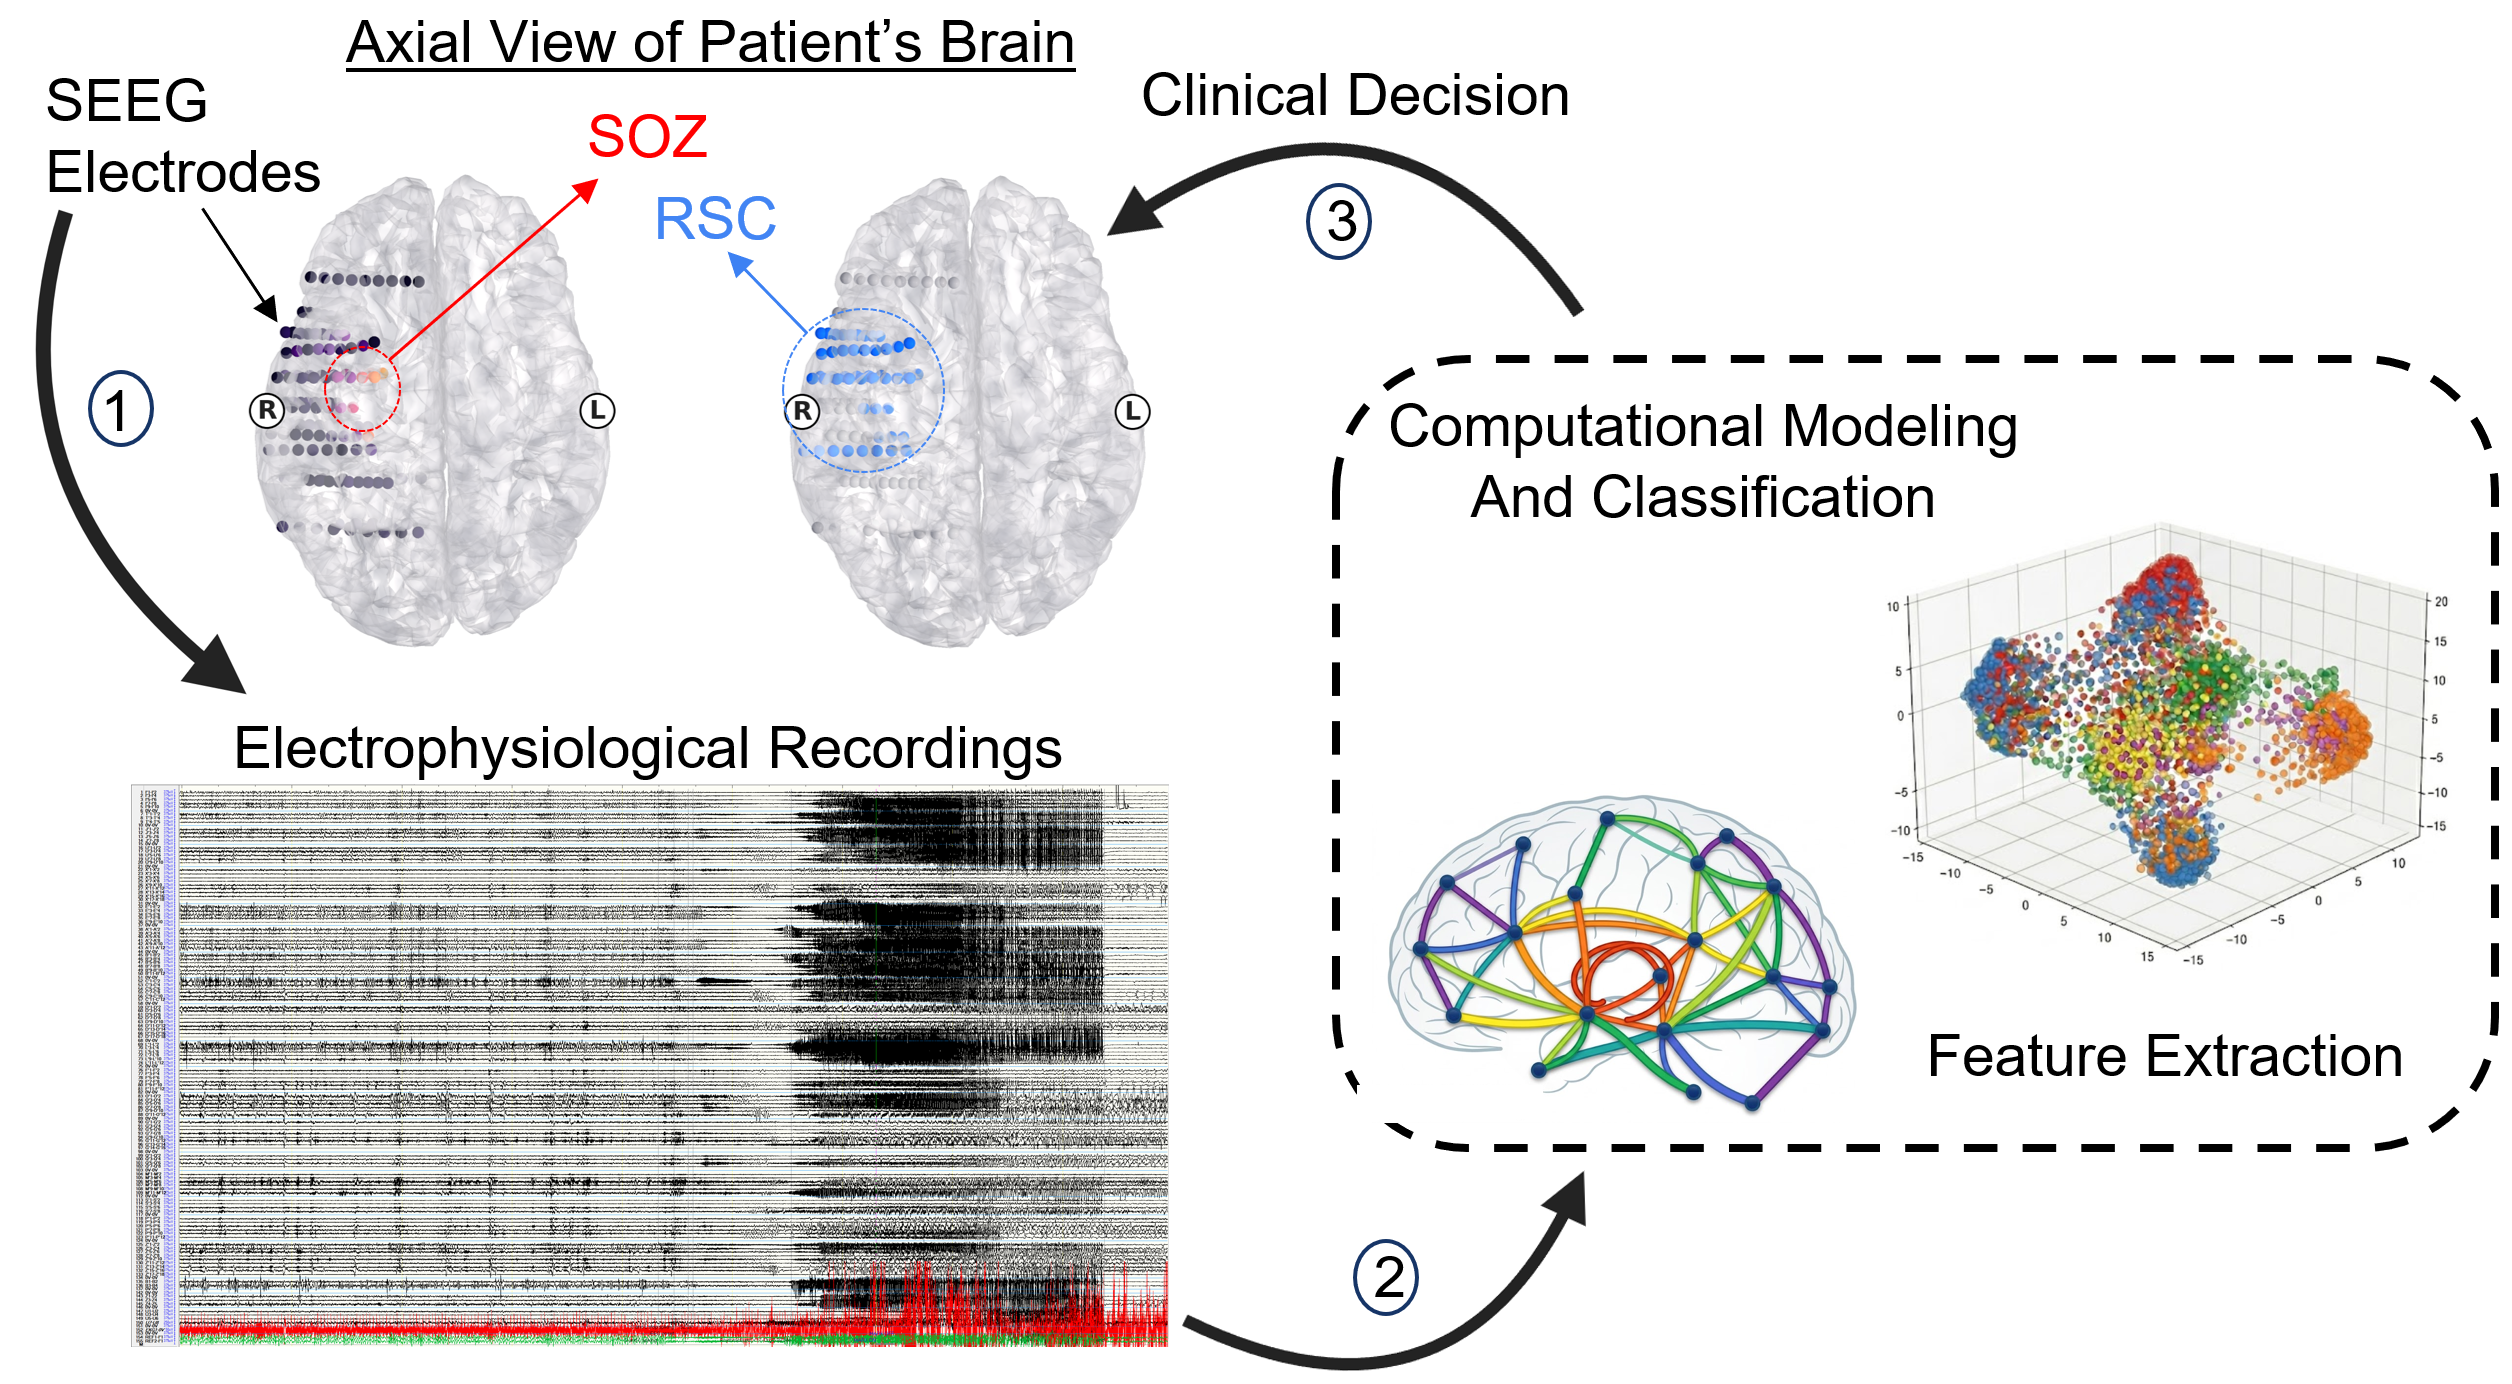
\includegraphics[width=\textwidth]{seeg_plot.png}
  \caption{\textbf{Overview of the SEEG-based functional connectivity analysis
  pipeline.} (1) Multi-contact depth electrodes are stereotactically implanted and localized on the patient's MRI. The clinically defined SOZ (red electrodes) is identified through visual inspection of raw SEEG recordings by expert clinicians. (2) Recorded signals undergo feature extraction, FC metric computation, and classification to characterize network-level dynamics. (3) The resulting network-level output informs pre-surgical decision-making; surgical success is subsequently validated by confirming that the resected region (blue electrodes) encompasses the identified SOZ post-operatively. (MRI = magnetic resonance imaging; RSC = resected region; SOZ = seizure onset zone)}
  \label{fig:seeg_overview}
\end{figure}


Increasing evidence suggests that epilepsy is better understood as a disorder of distributed brain network activity rather than as a purely focal abnormality \cite{spencer2002neural, kramer2012epilepsy}. Seizures emerge from abnormal and often hypersynchronous interactions among multiple brain regions, shaping seizure initiation, propagation, and clinical semiology \cite{bartolomei2017defining, murray2024network, da2003epilepsies}. Within this framework, several epilepsy-related zones have been described, including the irritative zone, seizure onset zone, epileptogenic zone, propagation zone, and symptomatogenic zone \cite{Jehi2018-jc}. In presurgical evaluation, these zones must also be considered with relation to the eloquent cortex, where resection carries a risk of functional impairment. The epileptogenic zone (EZ), as a theoretical concept, is the region directly responsible for the earliest organization/generation of seizure activity, whereas the ictal/seizure onset zone (SOZ) is a clinical surrogate defined by the site or network in which seizures are first recorded electrographically \cite{Jehi2018-jc}. 

Stereoelectroencephalography (SEEG) is a minimally invasive recording technique that records neuronal activity directly from superficial and deep cortical as well as subcortical structures of the brain \cite{Serletis2014-em,Kondylis2025-xp,bulacio2016stereoelectroencephalography, mullin2016seeg}. Pioneered by Bancaud and Talairach, it has become a cornerstone of presurgical evaluation in drug-resistant focal epilepsy \cite{Bancaud1965, Talairach1966, gonzalez2013stereoelectroencephalography}. Unlike electrocorticography (ECoG), which primarily samples the cortical surface using subdural grids or strip electrodes \cite{Kuruvilla2003-us}, SEEG uses stereotactically implanted multi-contact depth electrodes to sample distributed superficial and deep brain regions simultaneously, typically over several days at sampling rates of 1--4\,kHz \cite{mullin2016seeg}. Its high temporal resolution, favorable signal-to-noise characteristics, reduced sensitivity to volume conduction, and access to deep brain structures make SEEG particularly well suited for anatomy-based functional connectivity analysis in epilepsy \cite{bartolomei2017defining, lagarde2018interictal} (Figure~\ref{fig:seeg_overview}).

Functional connectivity (FC) quantifies statistical dependence or temporal correlation between electrophysiological signals recorded from spatially separated anatomical locations \cite{friston1994functional,bastos2016tutorial}. It is distinct from structural connectivity, which refers to the physical architecture and connections of white-matter tracts \cite{yeh2021mapping}, while effective connectivity (EC) extends FC to directed, causal inference \cite{friston2011functional}. In this review, we consider both non-directed and directed approaches because both are widely used in the SEEG literature to characterize epileptic networks. Figure~\ref{fig:fc_class} provides an overview of FC methods commonly used in SEEG studies, highlighting their organization into non-directed and directed connectivity frameworks.  

Historically, early investigations of inter-regional brain interactions relied primarily on correlation-based techniques that quantified statistical dependencies between electrophysiological signals in time-domain \cite{Brazier1952-fd}. As interest shifted towards the oscillatory mechanisms underlying neural interactions, coherence-based approaches were adopted to characterize frequency-specific synchronization between brain regions \cite{Brazier1972-xt,Bartolomei1999-xa}. Subsequent methods like imaginary coherence and lagged coherence were developed to address methodological challenges associated with common-source effects and volume conduction \cite{Goodale2020-lj,Nolte2004-rx,Pascual-Marqui2007-zi}. In parallel, phase-based metrics, including phase-locking value (PLV) and phase-lag index (PLI) were being integrated to characterize oscillatory phase synchronizations \cite{lachaux1999measuring,Vinck2011-tv}.

\begin{figure}[t!]
  \centering
  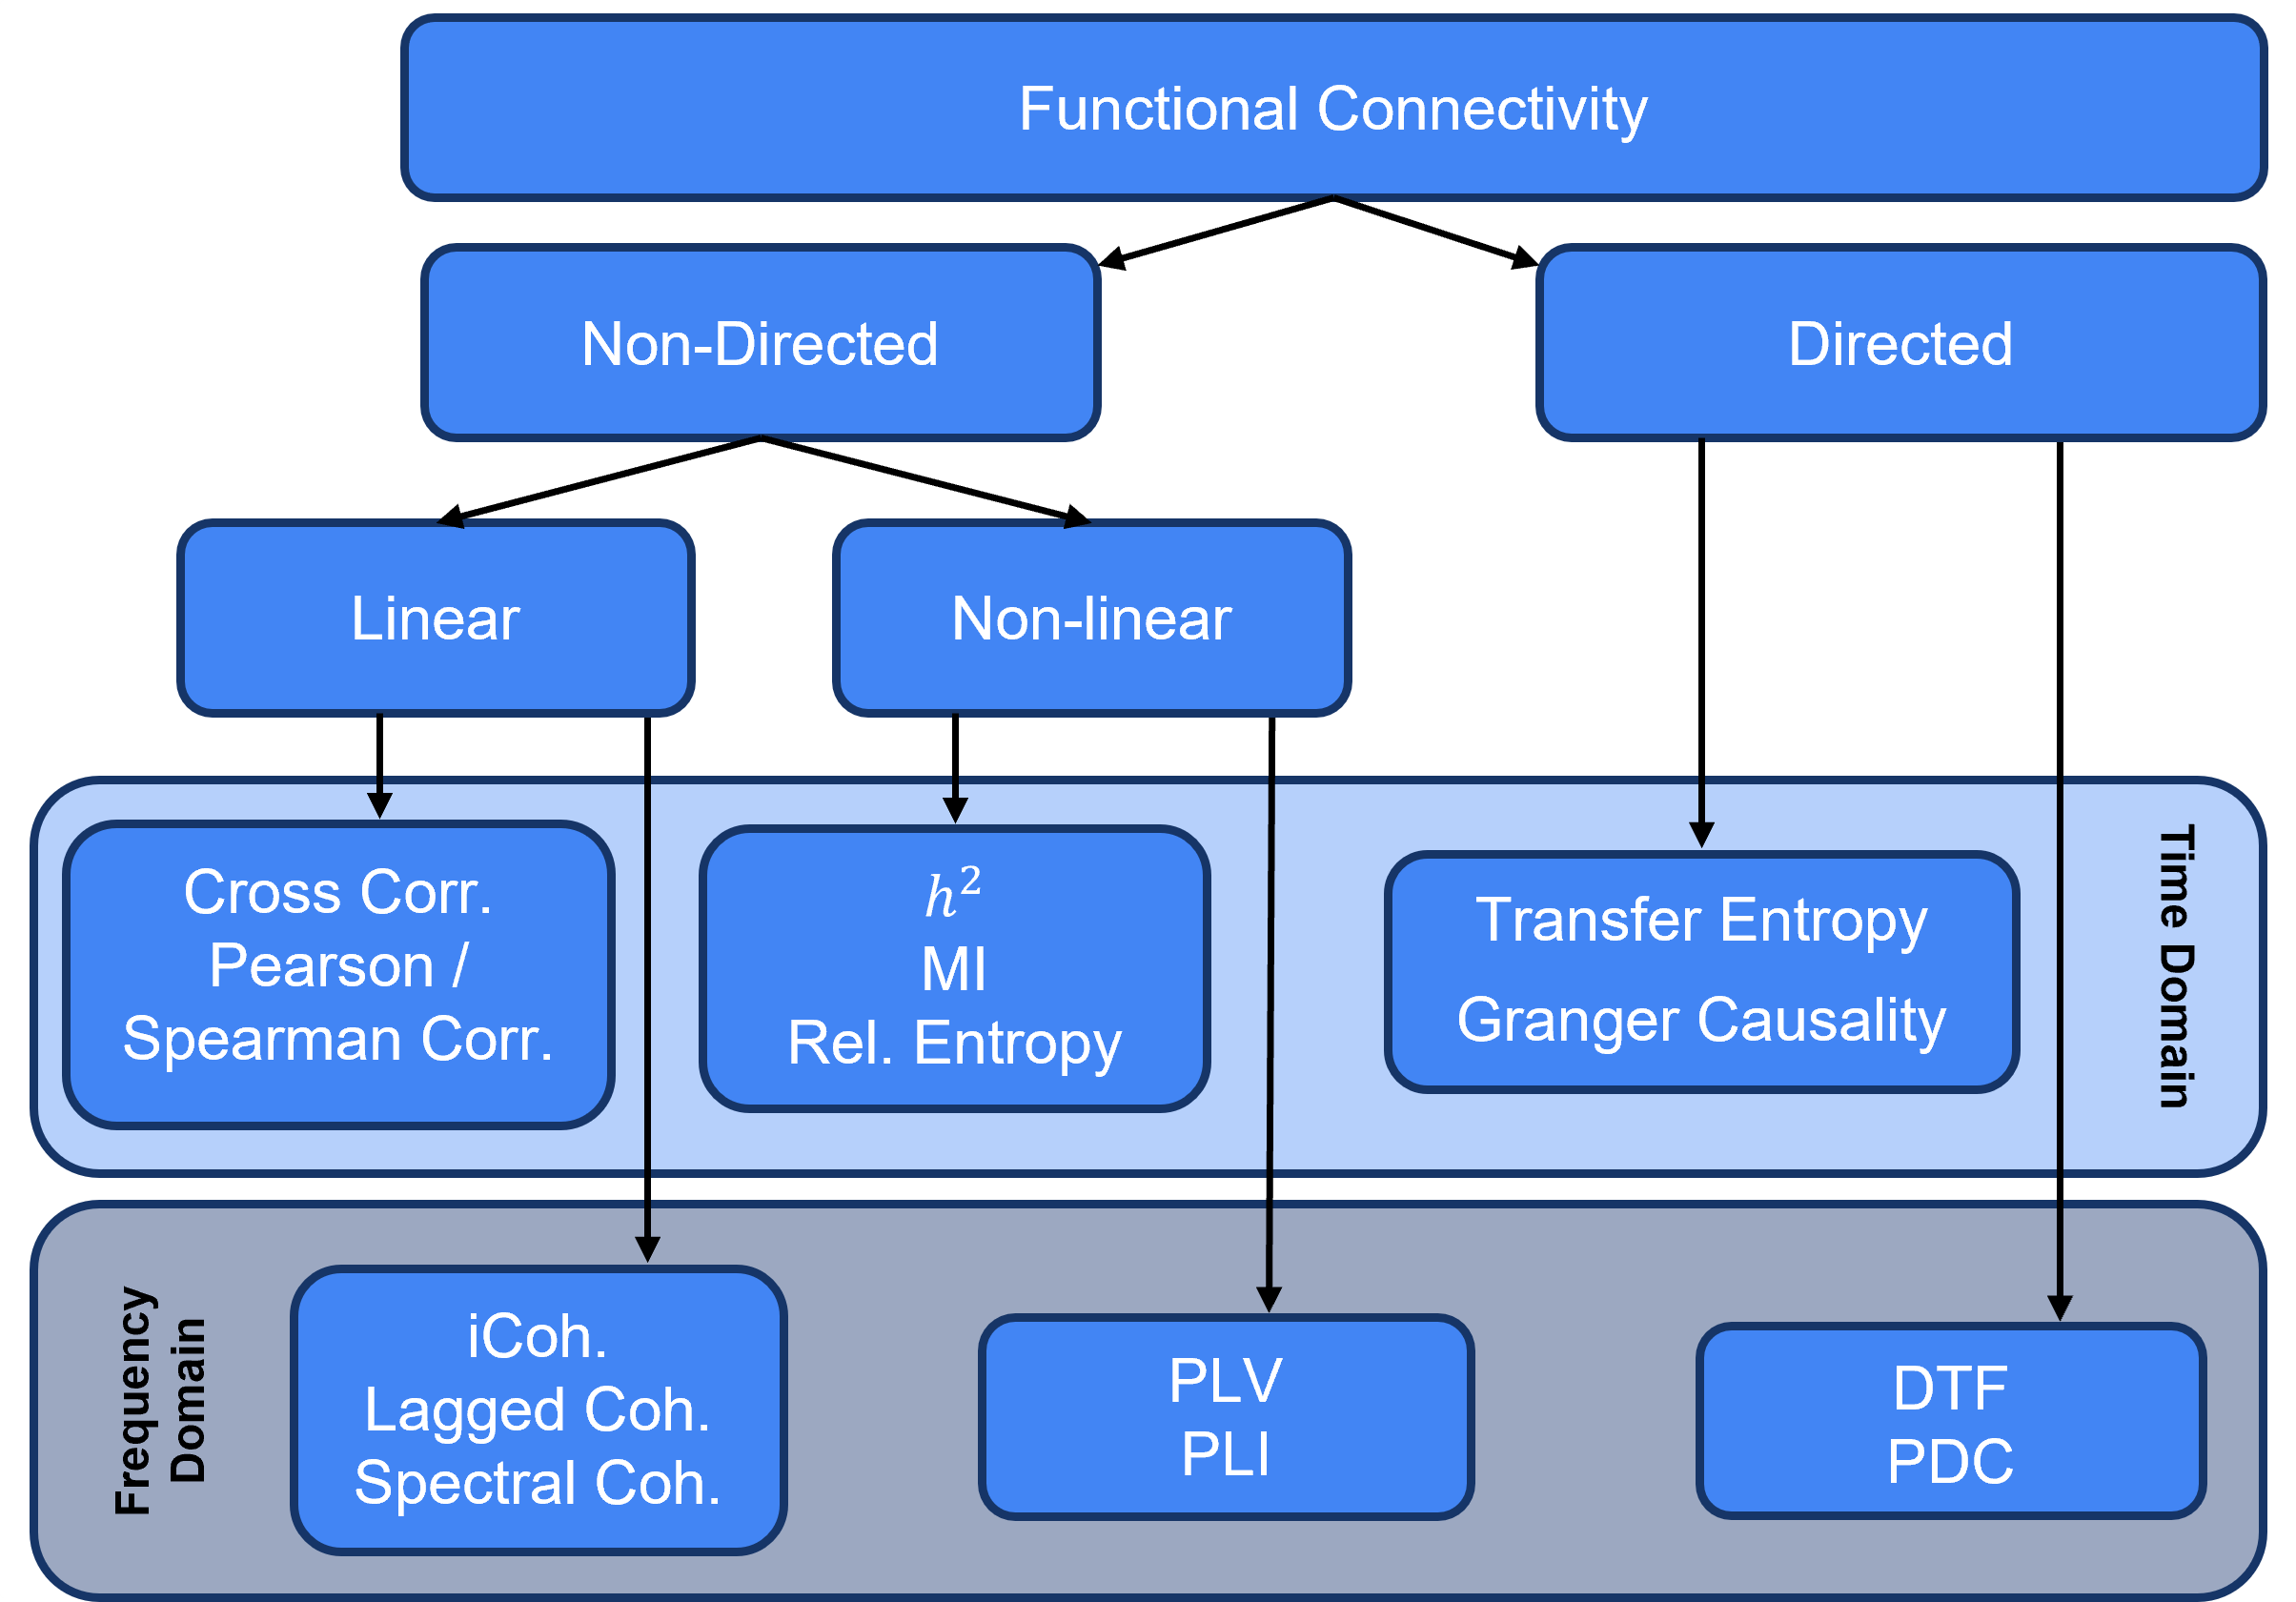
\includegraphics[width=0.65\textwidth]{FC_classification.png}
  \caption{\textbf{Taxonomy of functional connectivity measures used in SEEG analysis.} Metrics are divided into non-directed and directed connectivity. Each measure is then subdivided by linearity and by time-versus-frequency domain estimation. Non-directed linear time-domain measures include Pearson and cross-correlation; non-linear time-domain measures include $h^2$, mutual information, and relative entropy; frequency-domain measures include coherence variants (linear) and PLV/PLI (non-linear). Effective connectivity comprises directed time-domain measures (transfer entropy, Granger causality) and their frequency-domain derivatives (DTF, PDC). ($h^2$ = nonlinear regression; PLV = phase-locking value; PLI = phase-locking index; DTF = directed transfer function; PDC = partial directed coherence)}
  \label{fig:fc_class}
\end{figure}

Increasing recognition of epilepsy as a distributed network disorder further motivated the adoption of non-linear approaches capable of capturing interactions that may not be adequately described by linear dependence alone \cite{Casdagli1997-eh, John2025-hm}. Methods such as non-linear regression ($h^2$), mutual information, and relative entropy are therefore adopted to quantify more complex statistical relationships between neural signals \cite{Pallares_Di_Nunzio2026-xe, Lopes_da_Silva1989-nn,Wendling2001-te,Jeong2001-ni,Quiroga2000-eg}. While these methods characterize the presence and strength of interactions, they do not establish the direction of information flow between brain regions. This motivated the use of directed connectivity approaches influenced by Granger Causality \cite{Shojaie2022-ko} and its frequency-domain extensions, directed transfer function (DTF) and partial directed coherence (PDC), as well as information-theoretic measures such as transfer entropy \cite{Seth2015-fv,noauthor_undated-dv,Kaminski1991-pn,baccala2001partial}. Together, these methods provide complementary perspectives on epileptic networks by characterizing statistical dependence, oscillatory synchronization, non-linear interactions, and directed information transfer. A methodological overview of the described FC techniques is summarized in Supplementary Table~\ref{S-tab:FC_table}. 

From a signal-processing stand-point, the choice of FC metric influences the network representation that is ultimately observed, as different methods emphasize distinct aspects of neural interactions including statistical dependence, oscillatory synchronization, and/or directed information flow \cite{Lithari2012-lh}. This consideration is particularly important in SEEG because neural activity consists of heterogenous temporal states, ranging from relatively quiescent interictal periods to rapidly evolving ictal dynamics. Despite the growing body of work in this area, two important questions remained unresolved: what does the available evidence reveal about epileptic network organization in drug-resistant focal epilepsy (DRFE), and which findings are sufficiently robust to inform clinical practice? To address this gap, we examine the literature across five dimensions:

\begin{enumerate}
  \item \textbf{Methodological landscape and temporal trends:} Which FC measures have been applied to SEEG, how have they been evaluated clinically, and how has their use evolved between 2010 and 2025?

  \item \textbf{Method--epoch alignment:} How does the choice of FC measure vary across recording epochs (sleep, interictal, resting-state, preictal, ictal, and peri-ictal), and what patterns emerge from these pairings?

  \item \textbf{Frequency-band specificity:} Which frequency bands most consistently distinguish the SOZ from surrounding tissue, and does this vary by recording epoch?

  \item \textbf{Diagnostic performance for SOZ localization:} How accurately do FC measures identify the SOZ, and which analytical configurations show the strongest validation?

  \item \textbf{Prediction of surgical outcome:} To what extent do FC metrics predict postsurgical seizure freedom, and what factors appear to influence predictive performance?

\end{enumerate}


% ============================================
% 2. METHODS
% ============================================
\section{Materials and Methods}

\subsection{Search strategy}

We conducted a systematic search of Scopus, PubMed, and Web of Science for studies published between January 2010 and December 2025, with language restricted to English. The search strategy was: 

\begin{center}
\textit{(Functional AND Connectivity) AND 
((Intracranial AND EEG) OR (iEEG) OR 
(stereo AND electroencephalography) OR (SEEG))
}
\end{center}

The study selection followed PRISMA 2020 guidelines \cite{page2021prisma}. This time window captures approximately 15 years of methodological development in SEEG-based connectivity analysis. Foundational reviews of FC theory are available elsewhere \cite{bastos2016tutorial, bartolomei2017defining, Stergiadis2023-fl}. Most recently Almeida and Cunha \cite{Almeida2026-zi} provided a comprehensive review of SEEG-based functional and effective connectivity methods, focusing on their mathematical foundations, computational requirements, and methodological assumptions. In parallel, a recent ILAE Task Force systematic review and meta-analysis evaluated the broader literature on intracranial EEG connectivity in epilepsy surgery \cite{Sinha2026-mu}. The present review complements these efforts by focusing specifically on the clinical and biological insights derived from SEEG connectivity studies, examining how FC analysis has contributed to our understanding of epileptic network organization, seizure generation and propagation, SOZ localization, and surgical decision-making, while also identifying methodological factors that continue to limit clinical translation. 

\subsection{Eligibility criteria}
Studies were eligible if they were original peer-reviewed articles involving adult human participants who underwent clinical SEEG evaluation, applied at least one quantitative FC measure to SEEG recordings, and addressed epilepsy as the primary clinical focus. We excluded reviews and other non-research articles, exclusively paediatric cohorts ($<16$ years; excluded due to the ongoing large-scale network re-organization that introduces developmental variability not directly comparable with mature brain networks \cite{Spear2013-cd,Power2010-pl}), animal studies, purely computational models, stimulation-based paradigms including cortico-cortical evoked potentials and deep brain stimulation, task-based studies, non-invasive-only modalities without concurrent SEEG, cohorts with fewer than three patients, and studies focused solely on software development or algorithm benchmarking.

\subsection{Study selection and data extraction}
Records were imported into Zotero for aggregation and deduplication \cite{behera2022zotero}. Screening was performed independently by two reviewers in two stages: first by title and keyword, and then by abstract. Disagreements were resolved by consensus or, when necessary, by consultation with a third reviewer. Full-text articles were then assessed against the predefined eligibility criteria. Data were extracted using a standardized form that captured study metadata, clinical demographics, electrophysiological parameters, analytical methods, and reported clinical outcomes. Because of substantial heterogeneity in study design, patient populations, recording protocols, and analytical approaches, a descriptive synthesis was performed rather than a formal meta-analysis.

A total of 996 records were identified. After removal of 357 duplicates, 639 records underwent title and keyword screening, of which 339 were excluded. The remaining 300 records were screened by abstract, and 119 were excluded at this stage. Full texts were assessed for 181 articles, of which 120 did not meet the inclusion criteria. This yielded a final sample of 61 studies (Figure~\ref{S-fig:prisma}).


% ============================================
% 3. RESULTS
% ============================================
\section{Results}

\subsection{Study landscape}
Publication output increased markedly over the review period. Early work between 2010 and 2018 was relatively sparse, but the field expanded rapidly thereafter, with 31 of the 61 included studies (51\%) published in the final three years (2023--2025). This growth likely reflects both wider clinical adoption of SEEG and the maturation of network-based and graph-theoretical approaches. Study objectives also broadened over time. SOZ localization remained the most common aim (33\%), followed by peri-ictal dynamics (28\%), region-specific connectivity (23\%), surgical outcome prediction (10\%), and multimodal basic-science investigations (7\%) (Table~\ref{tab:seeg_studies}).


% ============================================
% TABLE 2: STUDY OVERVIEW
% ============================================
\begin{landscape}
  \typeout{LANDSCAPE LINEWIDTH = \the\linewidth}
  \setlength{\LTcapwidth}{\linewidth}
  \fontsize{7pt}{9pt}\selectfont
  \renewcommand{\arraystretch}{1.4}
  \setlength{\tabcolsep}{2pt}
  \begin{longtable}{
    >{\raggedright\arraybackslash}p{2.7cm}      % Authors (Year)
    >{\centering\arraybackslash}p{1.1cm}      % # Pts
    >{\centering\arraybackslash}p{1.2cm}      % Mean Age
    >{\centering\arraybackslash}p{1.2cm}      % # Sz
    >{\centering\arraybackslash}p{1.3cm}      % Seizure Type
    >{\centering\arraybackslash}p{2cm}        % Temporal Epochs
    >{\centering\arraybackslash}p{1.7cm}      % SEEG Window Length   
    >{\centering\arraybackslash}p{1.9cm}      % Modalities      
    >{\centering\arraybackslash}p{1.9cm}      % SEEG Sampling Rate
    >{\centering\arraybackslash}p{1.2cm}      % Multi-center    
    >{\centering\arraybackslash}p{2cm}        % Frequency Bands 
    >{\centering\arraybackslash}p{2.4cm}      % FC Metric
    >{\centering\arraybackslash}p{1cm}        % Follow-up (mo)
    }
\caption{Summary of SEEG and functional connectivity studies.}
\label{tab:seeg_studies} \\
\toprule
\textbf{\makecell[c]{Authors \\ (Year)}} &
\textbf{\# Pts} & \textbf{Mean Age} & \textbf{\# Sz} &\textbf{Seizure Type} & \textbf{Temporal Epochs} & \textbf{SEEG Window Duration} & \textbf{Modalities} & \textbf{SEEG Sampling Rate (Hz)} & \textbf{Multi-center} & \textbf{Frequency Bands} & \textbf{FC Metric} &
\textbf{Follow-up (month)} \\
\midrule
\endfirsthead
\multicolumn{13}{c}{\tablename\ \thetable{} -- \textit{continued}}\\
\toprule
\textbf{\makecell[c]{Authors \\ (Year)}} &
\textbf{\# Pts} & \textbf{Mean Age} & \textbf{\# Sz} &
\textbf{Seizure Type} & \textbf{Temporal Epochs} & \textbf{SEEG Window Duration} & \textbf{Modalities} & \textbf{SEEG Sampling Rate (Hz)} & 
\textbf{Multi-center} & \textbf{Frequency Bands} & \textbf{FC Metric} &
\textbf{Follow-up (month)} \\
\midrule
\endhead
\midrule
\multicolumn{13}{p{\linewidth}}{\textit{* SOZ Localization; ** Surgical Outcome; *** Seizure Phenotyping/Detection} \hfill\textit{Continued on next page}} \\
\multicolumn{13}{p{\linewidth}}{\textit{$\delta$-Delta, $\theta$-Theta, $\alpha$-Alpha, $\beta$-Beta, $\gamma$-Gamma, R-Ripple, BB-BroadBand; M-Median}} \\
\multicolumn{13}{p{\linewidth}}{\textit{Follow-up: Duration of post-surgical outcome assessment}} \\
\multicolumn{13}{p{\linewidth}}{\textit{`` -- '' indicates not reported.}} \\
\endfoot
\bottomrule
\multicolumn{13}{p{\linewidth}}{\textit{* SOZ Localization; ** Surgical Outcome; *** Seizure Phenotyping/Detection} \hfill\textit{Continued on next page}} \\
\multicolumn{13}{p{\linewidth}}{\textit{$\delta$-Delta, $\theta$-Theta, $\alpha$-Alpha, $\beta$-Beta, $\gamma$-Gamma, R-Ripple, BB-BroadBand; M-Median}} \\
\multicolumn{13}{p{\linewidth}}{\textit{Follow-up: Duration of post-surgical outcome assessment}} \\
\multicolumn{13}{p{\linewidth}}{\textit{`` -- '' indicates not reported.}} \\
\endlastfoot

$^{***}$Bettus et al.(2011)  & 5  & 37.4 & 0 & TLE  & Resting State & 15min &SEEG, fMRI & 512 & No & $\delta$,$\theta$,$\alpha$,$\beta$,$\gamma$,BB  & P. Corr & - \\[1ex]
$^{**}$Antony et al.(2013)   & 23 & 16.9 & 0 & TLE  & Resting State & 90sec &SEEG & 200, 500, 1k & No & BB & PLI & 12\\ [1ex]
$^{***}$Van Diessen et al.(2013)   & 12 & 38.4 & 0  & TLE  & Resting State & 8.9sec & SEEG & 2k & No & $\delta$,$\theta$,$\alpha$,$\beta$,$\gamma$,BB & $h^2$ & -\\[1ex]
$^{***}$Evangelista et al.(2015)   & 10 & 32.9 & 22 & TLE & Ictal & 2sec & SEEG & 256 & No & BB & $h^2$ & - \\ [1ex]
$^{*}$Courtens et al.(2016)  & 12  & 34.7 & 24  & Mixed & Preictal & 4sec & SEEG & 256, 612, 1025 & No  & $\theta$,$\alpha$,$\beta$,BB  & Spectral Coh.  & -\\[1ex]
$^{***}$Vecchio et al.(2016) & 10  & 31.6  & 0  & Mixed & Resting State  & 3min & SEEG & 256 & No & $\delta$,$\theta$,$\alpha$,$\beta$  & PDC  & -\\[1ex]
$^{*}$Li et al.(2016) & 7 & 23.3 & 21 & Mixed & Peri-Ictal & 5sec & SEEG & 512 & No & BB & $h^2$ & 14\\[1ex]
$^{***}$Hagiwara et al. (2017) & 5 & 26 & - & Insular & Ictal  & 4sec & SEEG & 256 & No & BB  & Adaptive DTF & 8 \\[1ex]
$^{*}$Yang et al.(2018) & 10 & 16 & 19  & Mixed & Peri-Ictal & 0.5sec & SEEG & 512 & No & BB & Coh. & 24 \\[1ex]
$^{***}$Aupy et al.(2018) & 15 & 44.3 & 69 & TLE & Ictal & 5sec & SEEG  & -- & No & BB & P. Corr,  PLV & 19 \\[1ex]
$^{***}$Tauste Campo et al.(2018)  & 10 & 33.3 & 10 & TLE & Preictal & 0.6sec & SEEG & 500 & No & BB & $h^2$  & 28 \\[1ex]
$^{***}$Lagarde et al. (2018) & 59 & 24$^M$  & -  & Mixed  & Resting State  & 8sec & SEEG  &  256, 512, 1024 & No  & $\delta$,$\theta$,$\alpha$,$\beta$,$\gamma$  & $h^2$  & 48\\[1ex]
$^{***}$Aupy et al.(2019) & 11 & 27.45  & 22  & Mixed & Peri-Ictal  & 5sec & SEEG  & 1k & No  & $\delta$,$\theta$,$\alpha$,$\beta$,$\gamma$  & $h^2$  & -\\[1ex]
$^{***}$Wang et al.(2019) & 59  & 26.1  & 60  & TLE  & Peri-Ictal & 8sec & SEEG, PET  & 1k, 2k & No  & $\theta$,$\alpha$,$\beta$,$\gamma$,R  & MI & 18\\[1ex]
$^{*}$Coelli et al.(2019) & 7  & 22.7  & 7  & Mixed & Sleep, Peri-Ictal  & 16sec & SEEG  & 1k & No  & $\delta$,$\theta$,$\alpha$,$\beta$,$\gamma$  & Rel. Entropy  & -\\[1ex]
$^{*}$Klimes et al. (2019) & 30  & 34.2 & - & Mixed & Sleep States  & 1sec & SEEG & 2k & No & $\delta$,$\theta$,$\alpha$,$\beta$,$\gamma$,R & $h^2$ & 35\\[1ex]
$^{*}$Balatskaya et al.(2020) & 51 & 23.5 & 51 & Mixed  & Peri-Ictal & 3sec & SEEG & 256, 512, 1025 & No  & $\delta$,$\theta$,$\alpha$,$\beta$,$\gamma$ & PLV  & 84\\[1ex]
$^{***}$Frusque et al.(2020) & 9 & - & 27 & TLE & Peri-Ictal & 4sec & SEEG & 256 & No  & BB & Imag. Coh. & 19 \\[1ex]
$^{*}$Goodale et al. (2020) & 15 & 35.2  & -  & Mixed  & Resting State  & 1sec & SEEG & 1k & No & $\delta$,$\theta$,$\alpha$  & MI, Imag. Coh. PDC, DTF& 12\\[1ex]
$^{*}$Narasimhan et al.(2020) & 25 & 34.8 & - & Mixed & Resting State & 120sec & SEEG & 500, 1k& No & $\alpha$ & $h^2$ & 20 \\[1ex]
$^{***}$Fonti et al.(2021)  & 22 & 24.9  & 22  & Mixed  & Peri-Ictal  & 3sec & SEEG  & 256, 512 & No & BB & Cross-Frequency Coupling & 22 \\[1ex]
$^{**}$Li et al.(2021) & 16 & 32.6 & 36 & Mixed & Ictal & 1sec & SEEG & 512, 1024 & No & $\theta$,$\gamma$ & P. Corr  & 24  \\ [1ex]
$^{***}$Mo et al.(2021)  & 38  & 24   & - & TLE   & Sleep States  & 15sec & SEEG, MRI& 1k, 2k & No & $\gamma$ & $h^2$  & - \\[1ex]
$^{***}$Wang et al. (2021) & 45  & 18.85& 94& Mixed & Ictal & 23sec (avg) & SEEG, PET& 2k & No & $\delta$,$\theta$,$\alpha$,$\beta$    & P. Corr  & 12  \\[1ex]
$^{***}$Lopes et al.(2021)  & 10  & 23$^M$   & 29& TLE   & Peri-Ictal  & 2sec & SEEG, MEG& 1k, 2k & No & BB& Dynamic Network Modeling& - \\[1ex]
$^{*}$Gunnarsdottir et al.(2022) & 65  & 33.5 & 65& Mixed & Resting State  & 0.5sec & SEEG & 1k, 2k & Yes& BB& Imag. Coh. & 12  \\[1ex]
$^{***}$Jung et al.(2022) & 38  & 37.1 & 40& TLE   & Peri-Ictal     & 4sec & SEEG     & 256 & No & BB& Imag. Coh., PDC& 12  \\[1ex]
$^{*}$Paulo et al.(2022)  & 32  & 33.8 & - & Mixed & Resting State  & 120sec & SEEG     & 1k & No & $\alpha$ & MI & 18  \\[1ex]
$^{*}$Weiss et al. (2022)   & 35  & 32   & - & Mixed & Inter-Ictal    & 10-60min & SEEG     & 2k & Yes& R & DTF, Cross-Freq. Directionality & 12 \\[1ex]
$^{*}$Jiang et al. (2022)  & 27  & -    & - & Mixed & Resting State  & 10min & SEEG     & 1k, 2k & No & BB& Coh.     & 12  \\[1ex]
$^{***}$Chang et al.(2023) & 13  & 37.2 & 77& TLE   & Peri-Ictal     & 5sec & SEEG     & 2048 & No & $\beta$ & PLV& 12  \\[1ex]
$^{**}$Cousyn et al.(2023)  & 10  & 30.7 & - & Mixed & Resting State  & 20sec & SEEG     & -- & No & $\delta$,$\theta$,$\alpha$,$\beta$,$\gamma$  & $h^2$  & -   \\[1ex]
$^{**}$Hu et al.(2023)   & 53  & 23.1 & 53& Mixed & Peri-Ictal     & 2sec & SEEG     & 1k, 2k & No & $\delta$,$\theta$,$\alpha$,$\beta$,$\gamma$  & $h^2$  & 24  \\[1ex]
$^{*}$Li et al.(2023)   & 20  & -    & 49& Mixed & Inter/Pre/Ictal & 3sec & SEEG     & 1024 & No & $\alpha$,$\beta$,$\gamma$& Granger Causality & 12  \\[1ex]
$^{*}$Nahvi et al.(2023) & 7   & -    & 16& Mixed & Ictal  & 10sec & SEEG & 256 & No & BB& $h^2$  & 22  \\[1ex]
$^{***}$Simula et al.(2023) & 33  & 19   & - & Mixed & Inter-Ictal    & 5sec & SEEG     & 1024 & No & $\delta$,$\theta$,$\alpha$,$\beta$,BB & $h^2$  & -   \\[1ex]
$^{***}$Soulier et al.(2023) & 6   & 38   & 15& TLE   & Peri-Ictal     & 5sec & SEEG     & 512 & No & BB& P. Corr, Coh., PLV, PLI, MI     & -   \\[1ex]
$^{*}$Wang et al.(2023) & 15  & 28.6 & - & Mixed & Resting State  &  2.5sec & SEEG     & 2k & No & BB& Imag. Coh.     & 12  \\[1ex]
$^{**}$Xu et al.(2023)  & 10  & -    & 13& TLE   & Ictal &  1sec & SEEG     & 512 & No & $\delta$,$\theta$,$\alpha$,$\beta$,$\gamma$,BB  & $h^2$  & 24  \\[1ex]
$^{***}$Yang et al.(2023) & 20  & 19.4$^M$ & 20& Mixed & Peri-Ictal     & 2sec & SEEG     & 256, 512 & No & $\delta$,$\theta$,$\alpha$,$\beta$,$\gamma$  & $h^2$  & 36  \\[1ex]
$^{***}$Ye et al.(2023)   & 14  & -    & - & TLE   & Preictal & 2sec & SEEG     & 1k, 2k & No & $\beta$,$\gamma$,R     & Lagged Coh.    & -   \\[1ex]
$^{*}$Shahabi et al.(2023) & 16  & 31.2 & - & Mixed & Ictal & 1sec & SEEG     & 500 & No & $\gamma$,R  & Imag. Coh.     & 40  \\[1ex]
$^{***}$Doss et al.(2024) & 74  & 34.4 & 383  & Mixed & Peri-Ictal     & 5sec & SEEG     & 500 * No & $\delta$,$\theta$,$\alpha$,$\beta$,$\gamma$  & PDC& -   \\[1ex]
$^{***}$Doss et al.(2024) & 81  & 37.5 & - & Mixed & Resting State  & 120sec & SEEG     & -- & No & $\delta$,$\theta$,$\alpha$,$\beta$,$\gamma$  & DTF, Cross-Corr  & -   \\[1ex]
$^{***}$Krishnan et al.(2024)     & 10  & 23.7 & 24& Mixed & Peri-Ictal     & 5sec & SPECT, SEEG & 1k & No & $\delta$,$\theta$,$\gamma$& $h^2$  & 21  \\[1ex]
$^{***}$Soncin et al. (2024)& 23  & 33.5 & - & TLE   & Resting State  & -- & SEEG   & 1024 & No & $\delta$,$\theta$,$\alpha$,$\beta$,BB & Transfer Entropy  & -   \\[1ex]
$^{*}$Sun et al. (2024)  & 15  & -    & 46& Mixed & Ictal & 6sec & SEEG     & 1k & Yes& BB& P. Corr  & -   \\[1ex]
$^{*}$Vila-Vidal et al.(2024)    & 10  & 36.2 & 67& TLE   & Peri-Ictal     & 1sec & SEEG     & 250, 500 & No & $\delta$,$\theta$,$\alpha$,$\beta$,$\gamma$,BB  & PDC& 60  \\[1ex]
$^{*}$Yin et al.(2024)  & 12  & -    & 20& TLE   & Ictal & 1sec & SEEG     & 512 & No & $\gamma$,R  & $h^2$  & -   \\[1ex]
$^{***}$Zanello et al.(2024)  & 14  & 32.8 & 25& Mixed & Peri-Ictal     & 3sec & SEEG     & 256 & No & BB& P. Corr, Coh., Cross-Corr, PLV, Rel Entropy   & 6 \\[1ex]
$^{*}$Conrad et al.(2024)  & 47  &20$^M$  & - & TLE   & Sleep States    & 60sec & fMRI, SEEG  & 512-2048 & Yes& $\delta$,$\theta$,$\alpha$,$\beta$,$\gamma$,BB   & Coh.     & 12  \\[1ex]
$^{***}$Aung et al.(2025) & 9   & 32   & 148   & TLE   & Inter-Ictal, Ictal & 5sec & SEEG     & 2048 & No & $\delta$,$\theta$,$\alpha$,$\beta$,$\gamma$,R& $h^2$  & 16  \\[1ex]
$^{***}$Chibany et al.(2025)    & 31  & 32   & 68& Mixed & Peri-Ictal   & 10sec & SEEG  & 1k & No & BB& PAC, PLI, PLV, Spectral Coh., Cross-Corr, Pred. Error Conn. & 6 \\[1ex]
$^{**}$Ivankovic et al.(2025)   & 21  & 22$^M$   & 21& Mixed & Inter-Ictal, Ictal  & 1sec & SEEG & 250-2048 & No & $\delta$,$\theta$,$\alpha$,$\beta$,$\gamma$  & PLV  & 60  \\[1ex]
$^{***}$Li et al. (2025)  & 10  & -    & 24& TLE   & Peri-Ictal     & 3sec & SEEG     & 1024 & No & $\theta$,$\alpha$,$\beta$,$\gamma$    & DTF& -   \\[1ex]
$^{***}$Peng et al.(2025) & 11  & 40.1 &  11  & Mixed & Ictal & 2sec & SEEG     & 1k & Yes& $\beta$ & DTF& 12  \\[1ex]
$^{***}$Wang et al.(2025) & 14  & 35.7 & 52& TLE   & Peri-Ictal     & 1sec & SEEG     & 500, 1024 & Yes& $\delta$,$\theta$,$\alpha$,$\beta$,$\gamma$,R& PAC, DTF, wPLI& 6   \\[1ex]
$^{*}$Xu et al.(2025)   & 61  & 22   & - & Mixed & Preictal & 5sec & SEEG     & 1k & No & $\delta$,$\theta$,$\alpha$,$\beta$,$\gamma$,R& $h^2$  & -   \\[1ex]
$^{***}$He et al.(2025)   & 16  & 25.5 & 62& TLE   & Preictal & 2sec & SEEG     & $\leq$1k & Yes& $\delta$,$\theta$,$\alpha$,$\beta$,$\gamma$,R& Total Corr.-based Synchronization  & -   \\[1ex]
$^{***}$Li et al.(2025)   & 8   & 24.5 & 16& TLE   & Preictal & 20sec &  SEEG     & 1024 & No & $\beta$ & Transfer Entropy  & -   \\[1ex]
$^{***}$Hou et al.(2025)  & 9   & 28.1 & 9 & TLE   & Preictal, Ictal  & 2sec & SEEG     & 512 & No & BB& Transfer Entropy & - \\[1ex]
  \end{longtable}
\end{landscape}


\subsection{Temporal contexts of analysis}
The included studies examined SEEG connectivity across the full seizure cycle. Interictal recordings, defined as recordings obtained between seizures, included interictal discharge periods, resting-state recordings, and sleep recordings \cite{Janca2015-bu, Weiss2022-xy, Li2023-vy, Simula2023-lj, Aung2025-gz, Ivankovic2025-ng, Von_Ellenrieder2022-ei, Coelli2019-hu, Klimes2019-ie, Mo2021-ig, Conrad2024-uh}. Resting-state recordings were typically defined as interictal periods without overt epileptiform discharges, usually acquired with eyes closed and no task, often at least two days after implantation and four hours from the nearest seizure to reduce the effects of anesthesia and ictal changes \cite{Bettus2011-jh, Antony2013-jw, Van_Diessen2013-pr, Vecchio2016-dn, lagarde2018interictal, Goodale2020-lj, Narasimhan2020-af, Paulo2022-pt, Jiang2022-uq, Cousyn2023-fj, Wang2023-ys, Doss2024-rs, Soncin2024-iz}.

Peri-ictal recordings captured the transition from preictal states through the seizure itself and into postictal recovery \cite{Li2016-hi, Yang2018-yx, Aupy2019-je, Wang2019-jl, Coelli2019-hu, Balatskaya2020-vi, Frusque2020-bn, Fonti2021-dz, Lopes2021-sf, Jung2022-rx, Chang2023-bc, Hu2023-kr, Soulier2023-rr, Yang2023-xe, Doss2024-ce, Krishnan2024-sq, Vila-Vidal2024-ha, Zanello2024-ap, Chibany2025-ob, Li2025-os, Wang2025-ij}. In many studies, the preictal phase, typically defined as the minutes preceding seizure onset \cite{Courtens2016-zs, Tauste_Campo2018-ga, Li2023-vy, Ye2023-jm, Xu2025-lh, He2025-tw, Li2025-vh, Hou2025-es}, and the ictal phase, defined as the electrographic seizure itself \cite{Evangelista2015-dz, Aupy2018-au, Li2023-vy, Xu2023-rm, Yin2024-ls, Aung2025-gz, Ivankovic2025-ng, Hou2025-es}, were analyzed separately.

Across the included literature, peri-ictal recordings (31\%) were the most frequently studied temporal context, followed by ictal (22\%), resting states (21\%), preictal (12\%), and interictal (7\%), whereas sleep (6\%) was the least represented (Figure~\ref{fig:methods_overview}A).


\subsection{Cohort demographics, modalities, and data sourcing}
Included cohorts were generally small and heterogeneous, with a median of 15 patients per study (range 5--81) and a median age of 32 years (range 16--44) at the time of SEEG evaluation. In terms of epilepsy subtype, 41\% of studies focused exclusively on temporal lobe epilepsy, and a smaller number examined specific regions such as the insula \cite{Hagiwara2017-sz}. Most studies (57\%) included mixed cohorts spanning frontal, cingulate, insulo-opercular, and temporal epilepsies.

In 89\% of studies, functional connectivity was computed exclusively from SEEG recordings, while the remaining 11\% used multimodal designs that combined SEEG with magnetic resonance imaging (MRI) \cite{Mo2021-ig}, functional MRI (fMRI) \cite{Bettus2011-jh, Conrad2024-uh}, magnetoencephalography (MEG) \cite{Lopes_da_Silva2013-li}, positron emission tomography (PET) \cite{Wang2019-jl, Wang2021-iw}, or single-photon emission computed tomography (SPECT) \cite{Krishnan2024-sq}. These multimodal approaches were typically used to provide complementary anatomical, functional, or metabolic information.

Most studies were conducted at a single center, however, a small but growing number used public datasets or multicenter collaborations to test generalizability across more heterogeneous populations \cite{Gunnarsdottir2022-la, Weiss2022-xy, Sun2024-bj, Conrad2024-uh, Peng2025-nx, Wang2025-ij, He2025-tw}.


\subsection{Methodological landscape}
Across the 61 included studies, 16 distinct FC measures were identified and grouped into four broad methodological categories (Figure~\ref{fig:methods_overview}B). Individual studies applied between one and six measures. Overall, non-directed approaches accounted for most reported method applications (73\%). Among these, non-linear regression ($h^2$) was the single most frequently used metric, appearing in 33\% of studies \cite{Bettus2011-jh, Evangelista2015-dz, Courtens2016-zs, Hagiwara2017-sz, lagarde2018interictal, Aupy2019-je, Wang2019-jl, Balatskaya2020-vi, Fonti2021-dz, Wang2021-iw, Hu2023-kr, Li2023-vy, Simula2023-lj, Soulier2023-rr, Yang2023-xe, Ye2023-jm, Soncin2024-iz, Zanello2024-ap, Chibany2025-ob, He2025-tw} (Figure~\ref{fig:methods_overview}C). Notably, $h^2$ was used more frequently than mutual information, despite mutual information being capable of capturing both linear and non-linear dependencies. This preference may reflect methodological and practical considerations. Mutual information requires estimation of joint probability distributions, whose performance depends on sample size and estimator choice, while $h^2$ is computationally simpler and can provide stable estimates from relatively short SEEG segments (Table~\ref{S-tab:FC_table} in supplementary). Its continued use likely reflects its demonstrated sensitivity to non-linear interactions associated with seizure generation and propagation \cite{pijn1990localization}.

Other commonly used non-directed measures included PLV \cite{Frusque2020-bn, Cousyn2023-fj, Wang2021-iw, Conrad2024-uh, Ivankovic2025-ng, Li2025-os}, Pearson correlation \cite{Antony2013-jw, Tauste_Campo2018-ga, Mo2021-ig, Lopes2021-sf, Wang2023-ys, Vila-Vidal2024-ha, Conrad2024-uh}, imaginary coherence \cite{Goodale2020-lj, Jung2022-rx, Paulo2022-pt, Xu2023-rm, Doss2024-rs}, PLI \cite{Van_Diessen2013-pr, Wang2023-ys, Ivankovic2025-ng, Xu2025-lh}, and lagged coherence \cite{Shahabi2023-ak}. Directed measures accounted for 19\% of reported method applications and were led by DTF \cite{Narasimhan2020-af, Jiang2022-uq, Krishnan2024-sq, Peng2025-nx, Wang2025-ij, Xu2025-lh, Yang2018-yx} and PDC \cite{Li2016-hi, Paulo2022-pt, Doss2024-ce, Yin2024-ls}, whereas transfer entropy \cite{Sun2024-bj, Hou2025-es} and Granger causality \cite{Nahvi2023-lm} were less common. A smaller number of studies (9\%) extended beyond these standard approaches by using custom connectivity metrics \cite{Gunnarsdottir2022-la, Jiang2022-uq} or cross-frequency coupling measures to investigate interactions across frequency bands \cite{Li2021-gq}.

\begin{figure}[htbp]
  \centering
  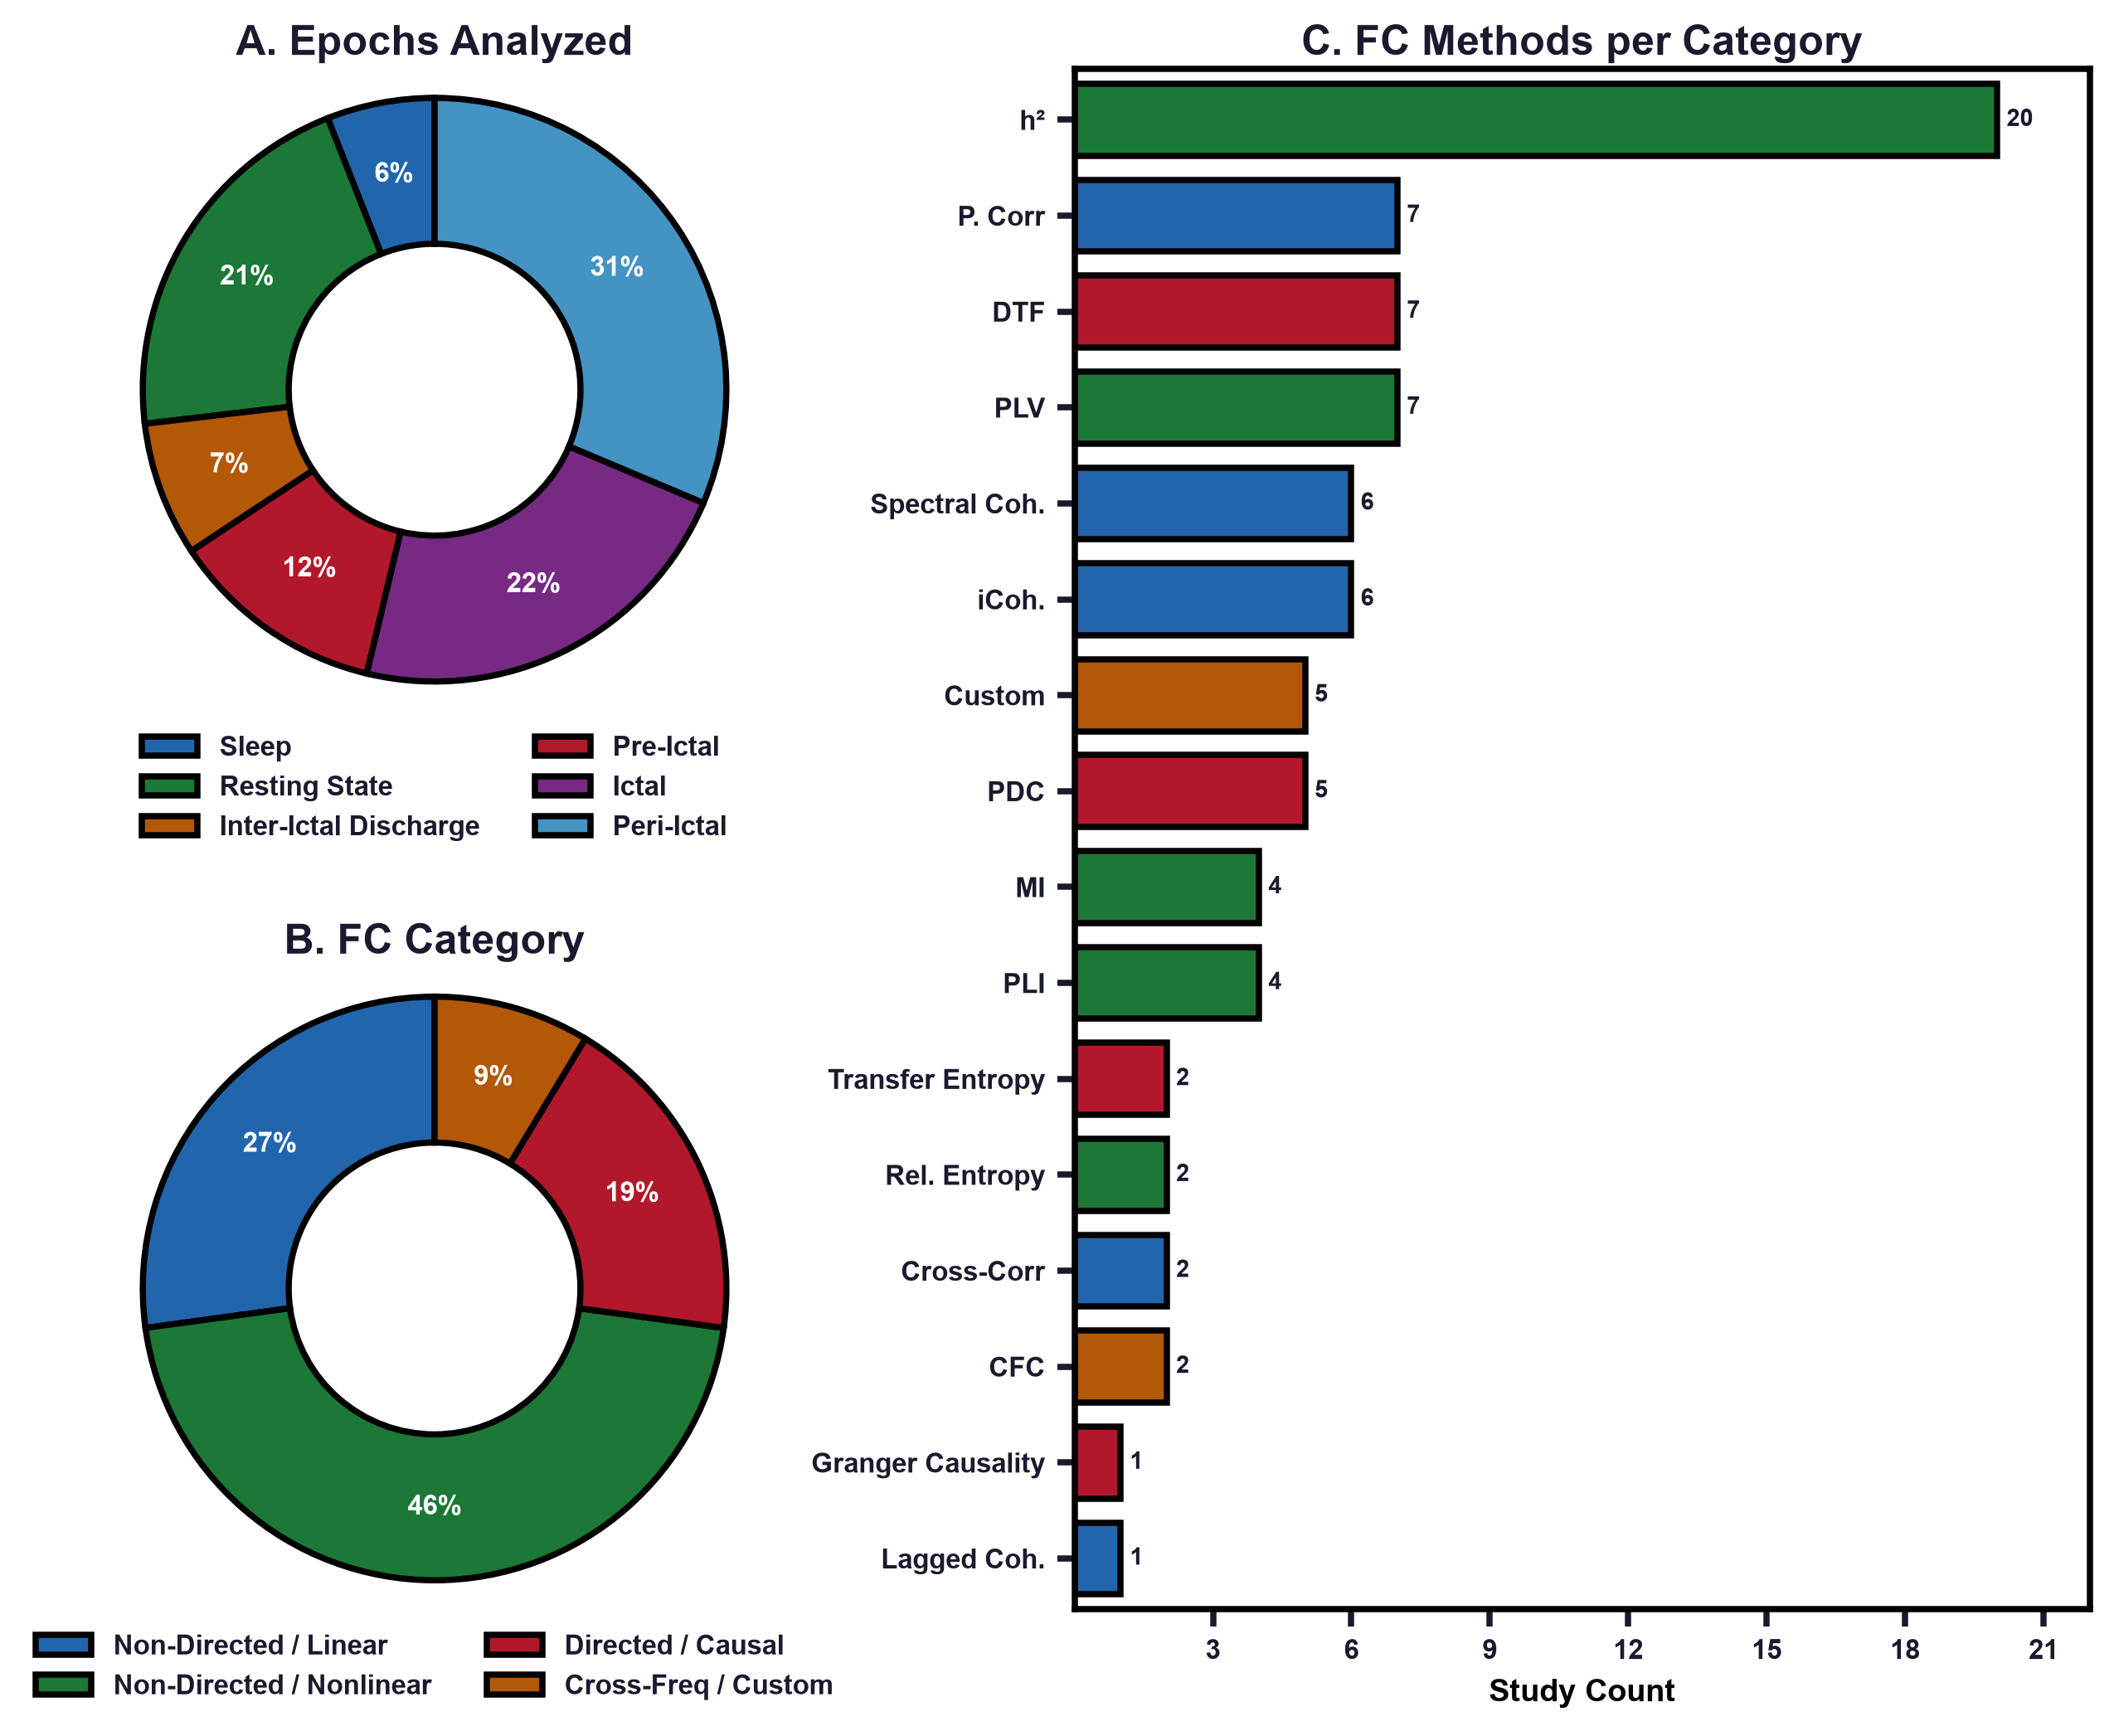
\includegraphics[width=\textwidth]{figure_03_methods_overview}
  \caption{\textbf{Functional connectivity methods across included studies.}
  (A) Distribution of analyzed epochs across studies; percentages
  refer to study--epoch instances, as individual studies could analyze more
  than one epoch. Peri-ictal recordings were the most frequently analyzed
  epoch (31\%), followed by ictal (22\%) and resting-state (21\%) recordings.
  (B) Distribution of study--method instances by FC category.
  Non-directed nonlinear methods accounted for nearly half of all instances
  (46\%). (C) Frequency of individual FC methods, color-coded by
  category as in (B). Non-linear regression ($h^2$) was used in 33\% of
  studies, more than any other single method.}
  \label{fig:methods_overview}
\end{figure}

Method choice varied with publication period, analytical window, and clinical objective (Figure~\ref{fig:overview}A--D). $h^2$ remained the most frequently used metric throughout the review period, peaking in 2023; however, from 2018 onward the methodological repertoire broadened considerably, with phase-synchrony (PLV, iCoh) and directed (DTF, PDC) measures appearing more regularly and information-theoretic and causal measures, such as transfer entropy, relative entropy, and Granger causality, emerging only from 2023 (Figure~\ref{fig:overview}A). This diversification likely reflects growing interest in network directionality and time-varying seizure dynamics. Across clinical objectives, SOZ localization drew on the full range of FC metrics, whereas other objectives relied on a narrower subset: $h^2$ dominated studies of region-specific dynamics, and studies of ictal dynamics most often used DTF and PLV (Figure~\ref{fig:overview}B). Metric use also differed by analytical window (Figure~\ref{fig:overview}C). $h^2$ was most strongly associated with peri-ictal analyses, which also employed linear, phase-based, and directed measures, while resting-state recordings were analyzed with the a broader set of metrics, including PDC, iCoh, MI, and PLI. Finally, analytical windows were linked to clinical objective (Figure~\ref{fig:overview}D): SOZ localization was the only objective studied across all six windows, studies of ictal dynamics focused on pre-ictal and peri-ictal recordings, region-specific dynamics were examined predominantly in peri-ictal data, and surgical outcome prediction drew on both resting-state and ictal recordings.

\begin{figure}[htbp]
  \centering
  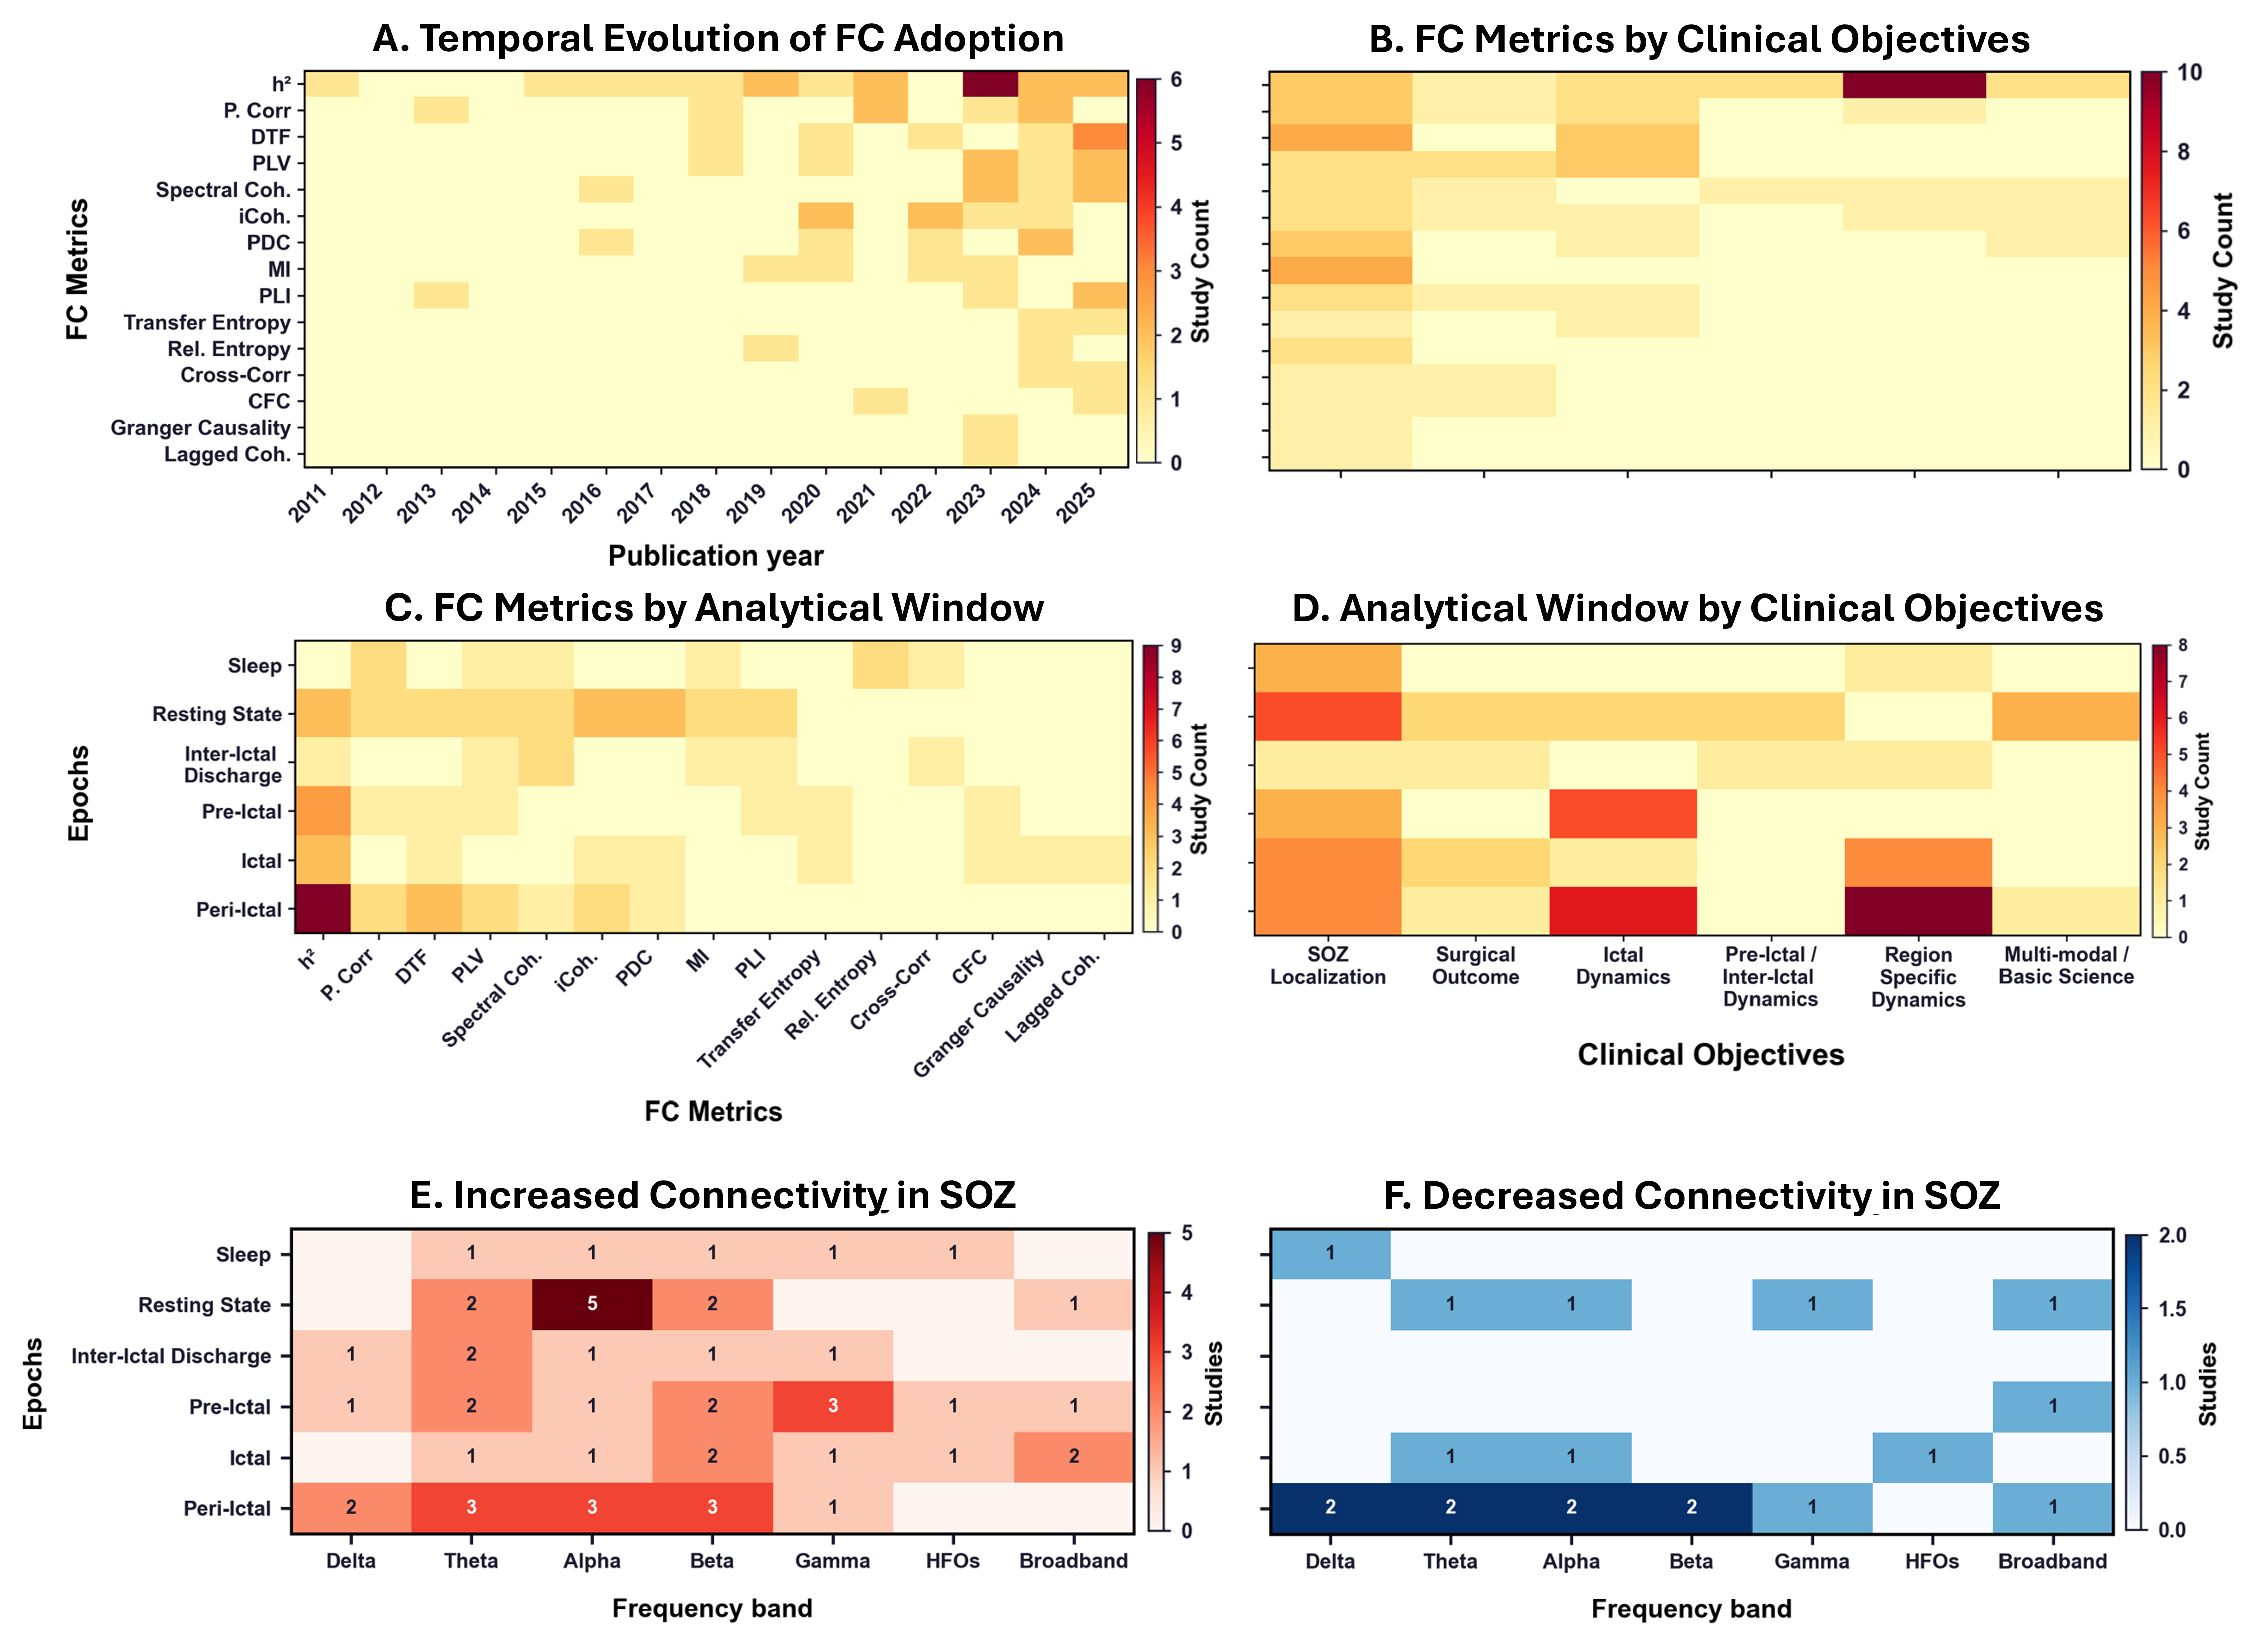
\includegraphics[width=\textwidth]{overview_epochs_metrics_objectives.png}
\caption{\textbf{Connectivity method use stratified by temporal context and clinical objective.} (A) Temporal evolution of FC metric adoption, 2011--2025. (B) FC metric use by
clinical objective; rows follow the metric order in (A) and columns the
clinical objectives in (D). (C) FC metric use by analytical window (epoch).
(D) Analytical window by clinical objective. In (A)--(D), color intensity
indicates the number of studies. (E, F) Number of studies reporting increased
(E) or decreased (F) connectivity within the SOZ, by analytical window and
frequency band. (SOZ: seizure-onset zone.)}

  \label{fig:overview}
\end{figure}

\subsection{Frequency-specific connectivity patterns across temporal contexts}
Across frequency bands, increased SOZ connectivity was the most common finding, although the consistency and direction of these effects varied by band and temporal context (Figure~\ref{fig:overview}E--F). Theta, alpha, and beta were the bands most often associated with increased SOZ connectivity across studies.

The theta band (4--8\,Hz), which has been linked to hippocampal function and seizure transition \cite{vertes2005hippocampal}, showed increased SOZ connectivity in 11 studies \cite{Vecchio2016-dn, Aupy2018-au, Coelli2019-hu, Cousyn2023-fj, Hu2023-kr, Krishnan2024-sq, Aung2025-gz, Ivankovic2025-ng, Li2025-os, Wang2025-ij, Xu2025-lh} and decreased connectivity in 4 \cite{Van_Diessen2013-pr, Wang2021-iw, Hu2023-kr, Vila-Vidal2024-ha}. Increased theta connectivity was especially prominent during interictal discharge periods, where decreases were not reported. The alpha band (8--12\,Hz), classically associated with relaxed wakefulness \cite{cantero2002human}, showed the most consistent resting-state pattern of any band, with 12 studies reporting increased SOZ connectivity \cite{lagarde2018interictal, Aupy2019-je, Coelli2019-hu, Goodale2020-lj, Narasimhan2020-af, Wang2021-iw, Paulo2022-pt, Hu2023-kr, Soncin2024-iz, Ivankovic2025-ng, Wang2025-ij, Xu2025-lh} and 4 reporting decreases \cite{Vecchio2016-dn, Hu2023-kr, Xu2023-rm, Vila-Vidal2024-ha}. One study \cite{Hu2023-kr} contributed to both groups, suggesting that directionality may depend on the analysis window or sub-band definition. The beta band (12--30\,Hz), often associated with active cognitive and motor processing \cite{kaminski2012beta}, showed increased SOZ connectivity in 11 studies \cite{Bettus2011-jh, Courtens2016-zs, lagarde2018interictal, Aupy2019-je, Coelli2019-hu, Wang2021-iw, Hu2023-kr, Xu2023-rm, Vila-Vidal2024-ha, Ivankovic2025-ng, Xu2025-lh} and decreased connectivity in 2 \cite{Hu2023-kr, Vila-Vidal2024-ha}. Beta-band effects were particularly prominent in preictal and ictal analyses.

Higher-frequency findings were somewhat less consistent but still informative. Gamma activity (30--100\,Hz), a marker of local cortical processing and a commonly studied SOZ feature \cite{Grinenko2018-zk}, was most often elevated in preictal analyses, with 7 studies reporting increases \cite{Coelli2019-hu, Li2021-gq, Vila-Vidal2024-ha, Ivankovic2025-ng, Li2025-os, Xu2025-lh, He2025-tw} and 2 reporting decreases \cite{Van_Diessen2013-pr, Vila-Vidal2024-ha}. High-frequency oscillations (HFOs; $>$100\,Hz), often considered highly specific markers of epileptogenic tissue \cite{Jacobs2012-uo}, were reported as increased in 3 studies \cite{Li2021-gq, Mo2021-ig, Li2023-vy}. By contrast, delta-band findings were the least consistent overall. Broadband analyses were most common in ictal studies but showed a mixed pattern, with similar numbers of increases and decreases. Sleep-related analyses also showed relatively diffuse and inconsistent band-specific effects.

The peri-ictal period showed the greatest complexity, with both increased and decreased SOZ connectivity reported across delta, theta, alpha, and beta bands. This pattern suggests substantial network reorganization around seizure onset and termination, with different methods capturing different aspects of the underlying dynamics.

\subsection{Classification and predictive performance}

Twenty-one studies (34\%) used formal classification approaches, including supervised models, unsupervised methods, and threshold-based heuristics (Table~\ref{tab:classification_studies}). Logistic regression was the most frequently used classifier \cite{Goodale2020-lj, Narasimhan2020-af, Wang2023-ys, Ye2023-jm, Xu2023-rm, Conrad2024-uh}, followed by support vector machines (SVM) \cite{Klimes2019-ie, Weiss2022-xy, Wang2023-ys, Yin2024-ls, Ivankovic2025-ng} and random forests \cite{Jiang2022-uq, Xu2025-lh}. More complex architectures, including a convolutional neural network \cite{Doss2024-rs} and a graph attention network \cite{Wang2025-ij}, appeared only in studies published after 2022. Unsupervised approaches, such as principal component analysis and clustering, were used to identify latent network structure without predefined labels.

Across studies using network-derived features, SOZ localization (15 studies) achieved a mean AUC of 0.79 (range 0.74--0.99), with mean sensitivity of 0.79 and mean specificity of 0.85 \cite{Klimes2019-ie,Balatskaya2020-vi,Goodale2020-lj,Narasimhan2020-af,Weiss2022-xy,Jiang2022-uq,Li2023-vy,Nahvi2023-lm,Wang2023-ys,Shahabi2023-ak,Sun2024-bj,Vila-Vidal2024-ha,Yin2024-ls,Conrad2024-uh,Xu2025-lh}. The two studies that focused on surgical outcome prediction \cite{Li2021-gq, Ivankovic2025-ng} reported a median AUC of 0.85 and four studies that classified network transitions for seizure predictions received AUC of 0.77 (range 0.75--0.9) \cite{Ye2023-jm,Doss2024-rs,Doss2024-ce,Wang2025-ij}. Comparative performance varied across studies. In one study, SVM and random forest performed best when applied to bivariate resting-state features \cite{Wang2023-ys}, whereas XGBoost performed best in a preictal setting using multiband higher-order features such as phase--amplitude coupling \cite{Xu2025-lh}. Taken together, these findings suggest that predictive performance depends more on feature construction and analytical context than on classifier family alone.


% ============================================
% TABLE 3: CLASSIFICATION STUDIES
% ============================================
\begin{landscape}
  \small
  \setlength{\LTcapwidth}{\linewidth}
  \fontsize{7pt}{9pt}\selectfont
  \renewcommand{\arraystretch}{1.5}
  \setlength{\tabcolsep}{4pt}
  \begin{longtable}{
    >{\raggedright\arraybackslash}p{3.5cm}
    >{\raggedright\arraybackslash}p{5.0cm}
    >{\raggedright\arraybackslash}p{2.8cm}
    >{\centering\arraybackslash}p{2cm}
    >{\centering\arraybackslash}p{2cm}
    >{\raggedright\arraybackslash}p{4cm}
    >{\raggedright\arraybackslash}p{2cm}
  }
  
%=================================================
% HEADER (FIRST PAGE)
%=================================================
  \caption{Summary of classification studies.}
    \label{tab:classification_studies} \\
    \toprule
    \textbf{Authors (Year)} & \textbf{Classification Model} &
    \textbf{Patient Outcome} & \textbf{Sensitivity} & \textbf{Specificity} &
    \textbf{Accuracy / AUC} & \textbf{Other Metrics} \\
    \midrule
    \endfirsthead
  %=================================================
  % HEADER (CONTINUATION PAGES)
  %=================================================
  \multicolumn{7}{l}{\tablename\ \thetable{} -- \textit{continued}}\\
    \toprule
    \textbf{Authors (Year)} & \textbf{Classification Model} &
    \textbf{Patient Outcome} & \textbf{Sensitivity} & \textbf{Specificity} &
    \textbf{Accuracy / AUC} & \textbf{Other Metrics} \\
    \midrule
    \endhead
  %=================================================
  % FOOTERS (empty: each category has its own legend)
  %=================================================
  \midrule
  \multicolumn{7}{@{}p{23cm}@{}}{%
  \renewcommand{\arraystretch}{1.3}%
  \begin{minipage}[t]{23cm}
  \tiny
  \textbf{Notation}\\[2pt]
  \begin{tabular}[t]{@{}ll@{\hspace{0.8cm}}ll@{\hspace{0.8cm}}ll@{\hspace{0.8cm}}ll@{}}
  *         & SOZ localization          & KNN & K-Nearest Neighbours         & cEI   & Connectivity Epileptogenicity Index                & PPV & Positive predictive value, $TP/(TP+FP)$ \\
  $\dagger$ & Highest model performance & SVM & Support Vector Machine       & CHFEI & Connectivity High-Frequency Epileptogenicity Index & NPV & Negative predictive value, $TN/(TN+FN)$ \\
            &                           & STE & Stepwise Transfer Entropy    &       &                                                    & FPR & False positive rate, $FP/(FP+TN)$ \\
  \end{tabular}
  \end{minipage}%
  }\\
  \endfoot
  %=================================================
  % FOOTER: LAST PAGE
  %=================================================
  \bottomrule
  \multicolumn{7}{@{}p{23cm}@{}}{%
  \renewcommand{\arraystretch}{1.3}%
  \begin{minipage}[t]{23cm}
  \tiny
  \textbf{Notation}\\[2pt]
  \begin{tabular}[t]{@{}ll@{\hspace{0.8cm}}ll@{\hspace{0.8cm}}ll@{\hspace{0.8cm}}ll@{}}
  **        & Surgical outcomes             & KNN & K-Nearest Neighbours          & AUC left  & AUC of Left side onset prediction  & PPV & Positive predictive value, $TP/(TP+FP)$ \\
  ***       & Seizure Phenotyping/Detection              & SVM & Support Vector Machine        & AUC right & AUC of Right side onset prediction & NPV & Negative predictive value, $TN/(TN+FN)$ \\
  $\dagger$ & Highest model performance     & PCA & Principal Component Analysis  &           &                                    & F2  & recall-weighted harmonic mean of PPV and sensitivity \\
            &                               & CNN & Convolutional Neural Network
  \end{tabular}
  \end{minipage}%
  }\\
  \endlastfoot

  % --------------- SOC localization -------->
  $^{*}$Klimes et al. (2019)          & SVM                                     & Engel$^{I,II,III,IV}$  & 0.89 & 0.71 & 0.9 (AUC)               & PPV = 0.56 \\[2ex]
  $^{*}$Balatskaya et al. (2020)      & cEI                                     & Engel$^{I,II,III,IV}$  & 0.79 & --   & 0.74 (AUC)              & PPV = 0.75 \\[2ex]
  $^{*}$Goodale et al. (2020)         & Linear Regression                       & --                     & 0.82 & 0.6  & 0.80 / 0.78             & -- \\[2ex]
  $^{*}$Narasimhan et al. (2020)      & Linear Regression                                   & Engel$^{I,II,III}$     & 0.79 & 0.81 & 0.84 / 0.88             & PPV = 0.46\newline NPV = 0.95 \\[2ex]
  $^{*}$Weiss et al. (2022)           & SVM                                     & Engel$^{I,II,III,IV}$  & 0.75 & 1    & 0.92 / 0.78             & PPV = 1\newline NPV = 0.9 \\[2ex]
  $^{*}$Jiang et al. (2022)           & Random Forest                           & Engel$^{I,II,III}$     & 0.8  & 0.9  & 0.92 / 0.93             & -- \\[2ex]
  $^{*}$Li et al. (2023)              & CHFEI  & -- & 0.79 & 0.84 & 0.85 / 0.88 & -- \\[2ex]
  $^{*}$Nahvi et al. (2023)           & Cross-Correlation of Outflow/Inflow     & Engel$^{I,II,III}$     & 0.5  & 0.94 & 0.9 (Acc.)          & -- \\[2ex]
  $^{*}$Wang et al. (2023)            & Linear Regression, Random Forest$^\dagger$, SVM$^\dagger$, KNN, Gasussian Naïve Bayes & Engel$^{I,II,III}$ & -- & -- & 0.84 (avg. Acc.)\newline 0.9 (avg. AUC) & -- \\[2ex]
  $^{*}$Shahabi et al. (2023)         & Unsupervised Clustering Algorithm       & Engel$^{I}$            & 0.88 & --   & --                      & FPR = 0.02 \\[2ex]
  $^{*}$Sun et al. (2024)             & STE                                     & --                     & 0.97 & 0.99 & 0.97 / 0.99             & -- \\[2ex]
  $^{*}$Vila-Vidal et al. (2024)      & Normalized Mean Activation$^\dagger$ \& Strength             & Engel$^{I,III}$ & -- & -- & 0.88 (mean AUC)    & F2 = 0.67 \\[2ex]
  $^{*}$Yin et al. (2024)             & DBO-SVM                                 & --                     & --   & --   & 0.96 (AUC)              & -- \\[2ex]
  $^{*}$Conrad et al. (2024)          & LASSO Linear Regression                 & Engel$^{I,II,III,IV}$  & --   & --   & 0.79/0.77 (AUC left)\newline 0.78/0.56 (AUC right) & -- \\[2ex]
  $^{*}$Xu et al. (2025)              & XGBoost$^\dagger$, CatBoost, AdaBoost, Logistic Regression, Random Forrest, Gasussian Naïve Bayes, KNN      & -- & 0.79 & 0.87 & 0.87 / 0.9 & -- \\[2ex]

  %--------------- Surgical Outcome ------->
  $^{**}$Li et al. (2021)             & Statistical Predictions                & Engel$^{I,II,III}$     & --   & --   & 0.8 (AUC)               & -- \\[2ex]
  $^{**}$Ivankovic et al. (2025)      & SVM                                    & Engel$^{I,II,III,IV}$  & 0.85 & 1    & 0.9 (AUC)               & -- \\[2ex]

  %------------- Seizure Phenotyping/Detection --------->
  $^{***}$Ye et al. (2023)            & Linear Regression                      & Engel$^{I}$            & --   & --   & 0.68 / 0.79             & -- \\[2ex]
  $^{***}$Doss et al. (2024)          & PCA (Unsupervised Learning)            & Engel$^{I,II,III,IV}$  & --   & --   & --                      & Prevalence Score = 0.79 \\[2ex]
  $^{***}$Doss et al. (2024)          & CNN                                    & --                     & 0.85 & 0.69 & 0.79 / 0.75             & -- \\[2ex]
  $^{***}$Wang et al. (2025)          & Graph Attention Network                & Engel$^{I}$            & 0.93 & 0.96 & 0.94 (Acc.)         & PPV = 0.97\newline NPV = 0.91 \\

   \end{longtable}
\end{landscape}




% ============================================
% 4. DISCUSSION
% ============================================
\section{Discussion}

Across 61 studies, SEEG-based functional connectivity analysis appeared capable of distinguishing epileptogenic from non-epileptogenic tissue and capturing seizure-related network dynamics. In studies reporting formal classification performance, SOZ localization achieved a mean AUC of 0.79, with mean sensitivity of 0.79 and specificity of 0.85, while smaller bodies of work suggests potential value for surgical outcome prediction with a mean AUC of 0.83 and seizure phenotype/detection with an AUC of 0.77 respectively. Taken together, these findings support SEEG-FC as a promising adjunct to conventional presurgical evaluation. In the following sections, we synthesize the evidence thematically and highlight both convergent and conflicting findings.


\subsection{The SOZ as a connectivity hub --- and the measure-specificity problem}
One of the most consistent findings across the reviewed literature is that the SOZ tends to show higher connectivity than surrounding tissue, particularly in the alpha, theta, and beta bands. This pattern has been reported across multiple temporal contexts and analytical frameworks. The largest resting-state study \cite{lagarde2018interictal} ($n=59$) provided strong evidence for persistent alpha- and beta-band hyperconnectivity within epileptogenic and propagation zones. Similar findings were reported by Goodale et al.\cite{Goodale2020-lj} and Narasimhan et al.\cite{Narasimhan2020-af}. Goodale et al. showed that within-SOZ connectivity decayed with electrode distance, suggesting a spatial organization not seen in non-SOZ tissue, whereas Narasimhan et al. reported increased inward-directed connectivity to the SOZ.

At the same time, this apparent consensus is complicated by an important methodological observation. Two studies \cite{Vila-Vidal2024-ha, Hu2023-kr} reported both increased and decreased connectivity within the same frequency band, depending on the FC measure used. This suggests that discrepancies across studies may not simply reflect noise or poor reproducibility, but also genuine differences in what individual metrics capture. Measures based on phase synchrony, amplitude coupling, and directed interactions are sensitive to different aspects of network organization. As a result, the same underlying neural process may appear as hyperconnected with one method and hypoconnected with another. Cross-study differences may also reflect biological and clinical heterogeneity, including variation in medication profiles \cite{Akkol_bc}, underlying pathology, seizure dynamotypes \cite{Saggio2020-sr}, and other patient-level confounders.

This has an important implication for the interpretation of SEEG-FC findings. Connectivity analysis is not simply a matter of applying a method to a dataset; the choice of metric shapes the biological phenomenon that becomes visible. Measure selection should therefore be guided by the clinical question, the temporal context of interest, and the specific aspect of neural dynamics under investigation. Greater attention to this issue will be essential for developing interpretable and reproducible connectivity-based biomarkers.

\subsection{Calibrating confidence across bands}
Forty-two studies reported band-specific findings, but not all of these carry the same weight. Findings replicated across multiple studies, methods, and centers provide stronger evidence than isolated observations. On this basis, increased alpha connectivity during resting-state recordings \cite{Goodale2020-lj, Narasimhan2020-af, Paulo2022-pt, Soncin2024-iz}, increased theta connectivity during peri-ictal periods \cite{Coelli2019-hu, Hu2023-kr, Krishnan2024-sq}, and increased preictal gamma connectivity \cite{Xu2025-lh, Li2025-os, Ivankovic2025-ng} appear to be among the most reliable signatures in the current literature.

By contrast, single-study findings such as decreased HFO connectivity during ictal recordings \cite{Xu2023-rm} or increased delta connectivity during interictal discharge periods \cite{Xu2025-lh} should be interpreted more cautiously until they are independently replicated. Delta-band findings deserve particular caution. Their inconsistency may reflect genuine biology rather than absence of effect, because conventional delta-band definitions exclude infraslow activity ($<0.5$\,Hz), which has been implicated in ictal and preictal state transitions \cite{Thompson2016-qs}. Accordingly, isolated findings should be regarded as preliminary, whereas candidate biomarkers require support across independent studies and analytical approaches.


\subsection{Directed dynamics: source--sink, Preictal reconfiguration, and terminal synchrony}
A central theme in the directed-connectivity literature is the source--sink model \cite{Gunnarsdottir2022-la}, in which the SOZ behaves as a sink during interictal periods by receiving inward influence, and then shifts toward a source at seizure onset. This interpretation is supported by several studies. Yang et al. \cite{Yang2018-yx} found that out-degree was a key discriminator of epileptic tissue during ictal recordings. In multimodal SEEG--SPECT work, Krishnan et al. \cite{Krishnan2024-sq} tracked outward information flow from the SOZ during the preictal period, followed by redirection toward hypoperfused regions at seizure onset and reversal as the seizure evolved. Xu et al. \cite{Xu2025-lh} further showed that inhibitory influence from regions outside the SOZ intensified as onset approached but ultimately failed, suggesting that seizure generation may reflect breakdown of network-level inhibition rather than a fixed local property alone. Importantly, these findings are most directly captured by directed measures, whereas non-directed methods cannot fully resolve the direction of information flow.

The preictal period appears to be a phase of active network reconfiguration rather than relative quiescence. Global FC decreases roughly 30 minutes before seizure onset \cite{Tauste_Campo2018-ga}, and alpha-band small-worldness is reduced \cite{Vecchio2016-dn}, suggesting departure from the interictal network state before electro-clinical onset. Clinical seizures have also been associated with stronger gamma-band and directed interactions within the SOZ than subclinical events \cite{He2025-tw}, indicating that seizure severity may be encoded in network topology before overt onset.

Several studies also converge on increased synchronization at seizure termination. Reported findings include elevated thalamo-cortical synchrony \cite{Evangelista2015-dz}, recruitment of the thalamus as a terminal receiver \cite{Soulier2023-rr}, similar late-stage involvement of cortico-striatal circuits \cite{Aupy2019-je}, and broader network integration during the late ictal phase \cite{Li2025-vh}. Although these findings were obtained using different measures, including $h^2$, coherence, correlation, and phase synchrony, they point to a recurring pattern of terminal network synchronization.

\subsection{Connectivity reflects circuit architecture and semiology}
FC measures appear to capture clinically meaningful information beyond SOZ localization alone. Several studies linked specific connectivity patterns to seizure semiology and regional circuit involvement. For example, oroalimentary automatisms were associated with stronger temporal-circuit connectivity \cite{Aupy2018-au, Wang2019-jl}, whereas patients with facial semiology showed increased alpha- and beta-band connectivity and reduced theta connectivity compared with patients with mesial temporal lobe epilepsy without facial semiology \cite{Wang2021-iw}. The insula also emerged as an important hub in frontal semiology through insula--mesial frontal coupling \cite{Hagiwara2017-sz}, and the striatum showed progressive engagement with the SOZ across the seizure cycle, peaking in the postictal period \cite{Aupy2019-je, Chibany2025-ob}.

SEEG also provides anatomical detail that is difficult to obtain with surface recordings. Depth-electrode studies identified reduced hippocampal--amygdala coupling in the high-gamma range in patients with hippocampal sclerosis \cite{Mo2021-ig}, as well as distinct connectivity profiles for ventral and dorsal amygdala subdivisions \cite{Aung2025-gz}. Together, these findings suggest that FC is sensitive not only to the distinction between epileptogenic and non-epileptogenic tissue, but also to the finer circuit architecture underlying specific seizure behaviors.


\subsection{Classification, label definition, window length, and evaluation}

Among the 21 studies that used formal classification approaches, SOZ localization was the most widely sought classification (15 studies) followed by those that sought to predict oncoming seizures and network transition changes (4 studies) and surgical outcome predictions (2 studies). logistic regression and support vector machines were the most commonly used classification tool, likely reflecting the small sample sizes typical of this literature. A shift toward more complex models is nevertheless apparent. Convolutional neural networks \cite{Doss2024-rs} and graph attention networks \cite{Wang2025-ij} appeared only after 2022, in parallel with the recent expansion of the field. The graph attention network is particularly well matched to SEEG-derived FC data because it operates directly on graph-structured connectivity matrices rather than requiring the adjacency matrix to be flattened into a conventional feature vector. However, both deep-learning studies were based on single-center datasets with fewer than 30 patients and lacked an independent hold-out cohort, limiting conclusions about generalizability. Unsupervised approaches, including PCA-based and agglomerative clustering \cite{Doss2024-ce, Shahabi2023-ak}, were also used to identify SOZ-related communities without predefined labels, which is especially relevant in SEEG because the reference labels themselves are derived from clinical consensus and are therefore inherently uncertain.

Window length is another important but often underemphasized analytical choice. Longer windows are better suited to capturing stable background organization, particularly in resting-state analyses, whereas shorter windows are more appropriate for resolving the transient network changes associated with seizure onset and termination. Coelli et al.\ \cite{Coelli2019-hu} showed that multiscale clustering localized the SOZ more effectively than any single window length alone. Because epileptic network dynamics span slow interictal fluctuations, rapid ictal transitions, and postictal suppression, no single window length is likely to be optimal across all contexts. Window selection should therefore be justified in relation to the temporal dynamics and clinical objective under study. Even so, some recurring method--context pairings have emerged in practice, including $h^2$ in peri-ictal localization, DTF in ictal dynamics, and phase-synchrony measures in resting-state analyses.

A further issue concerns the definition of ground-truth labels. In principle, three contact categories are available: the epileptologist-defined SOZ, the resected region (RSC), and the non-resected regions that were not considered as the SOZ. These categories are not interchangeable. The RSC is typically larger than the SOZ because surgical resections are often extended beyond the electrographically defined onset region in an effort to maximize seizure freedom \cite{Abdallah2026-ue,Vakharia2018-yx}. As a result, contacts located within the RSC but outside the SOZ occupy an ambiguous position and cannot be confidently assigned to either class.

This ambiguity has important consequences for classifier development. When RSC-but-not-SOZ contacts are treated as SOZ, label noise is introduced into the positive class, potentially degrading model training and inflating apparent SOZ specificity. We therefore recommend using epileptologist-defined SOZ contacts as positive labels and limiting negative labels to contacts outside both the SOZ and the resected region. Contacts within the resected region but outside the SOZ should be excluded from model training and evaluation. We note, however, that some of these excluded contacts may still contain SOZ-relevant activity.

Evaluation practices also require closer attention. SEEG datasets are typically highly imbalanced, with SOZ contacts representing only a small fraction of all sampled contacts \cite{Hrtonova2025-og}. Under these conditions, AUC-ROC can provide an overly optimistic picture because it is relatively insensitive to minority-class performance. The area under the precision--recall curve (AUPRC) is an important complementary metric because it more directly reflects the trade-off between positive predictive value and sensitivity in imbalanced settings \cite{Saito2015-kq}. None of the included studies reported AUPRC. Given the class imbalance inherent to SEEG contact labeling, we suggest that future studies report AUPRC alongside AUC-ROC as a minimum standard.

\subsection{Surgical outcome prediction}

Surgical outcome prediction is one of the most clinically important applications of SEEG-FC, although the available literature remains relatively limited. An early and influential finding was that patients with weak, spatially homogeneous connectivity were seizure-free in 90\% of cases, whereas patients with strong and heterogeneous connectivity showed seizure recurrence in 85\% of cases \cite{Antony2013-jw}. Subsequent studies have supported the broader idea that more spatially distributed and structurally constrained networks are associated with poorer outcomes. For example, unfavorable outcomes were linked to increased parieto-extra-parietal propagation connectivity \cite{Fonti2021-dz} and to stronger structural--functional coupling \cite{Chang2023-bc}, suggesting that resection may be less effective when epileptic activity is embedded within a broader anatomically constrained network.

Other studies suggest that seizure-free patients may show distinct ictal network signatures. Hu et al. \cite{Hu2023-kr} reported a transient decrease in FC during low-voltage fast activity at seizure onset, whereas Xu et al. \cite{Xu2023-rm} found that seizure-free patients showed dominant outward information flow from the surgical zone, in contrast to the inward-dominant pattern seen in patients who were not seizure-free. The most formally validated outcome-prediction model achieved an AUC of 0.903 using an iterative SVM-based network-state approach \cite{Ivankovic2025-ng}.

Taken together, these studies suggest that better outcomes may be associated with ictal networks that are more spatially focal, less tightly coupled to structural pathways, more weakly synchronized at onset, and characterized by outward rather than inward information flow. However, it remains unclear to what extent these features reflect the underlying biology of the epilepsy as opposed to differences in electrode sampling. Resolving this question will require prospective multicenter studies with more standardized implantation strategies and FC analysis pipelines.


\subsection{Limitations of the evidence base}
Beyond limitations inherent to any literature review, including publication bias and restriction to English-language studies, the primary literature has two recurring weaknesses that limit the strength of current conclusions. First, most studies were small and had relatively short follow-up: 80\% enrolled fewer than 30 patients, and the median follow-up duration was 18 months. This limits the ability to capture syndromic, surgical, and pathology-related heterogeneity and may underestimate delayed recurrence. Second, most studies were retrospective and single-center in design. Overall, 89\% were conducted at a single center, and prospective studies were absent, leaving the literature vulnerable to center-specific implantation practices and selection bias.


\subsection{Future directions and recommendations}

Building on the gaps identified above, we propose four practical recommendations for future SEEG-FC studies:
\begin{enumerate}
    \item \textbf{Select FC metrics on theoretical grounds.} Metric choice should be aligned with the clinical question and the specific neural dynamics of interest, rather than treated as a purely technical decision.
    \item \textbf{Report AUPRC alongside AUC-ROC.} Because SEEG datasets are strongly imbalanced at the contact level, evaluation should include metrics that are sensitive to minority-class performance.
    \item \textbf{Standardize ground-truth labeling.} Future studies should distinguish clearly among SOZ contacts, contacts outside both the SOZ and resected region, and ambiguous contacts within the resected region but outside the SOZ.
    \item \textbf{Prioritize prospective multicenter validation.} Broader validation with standardized implantation strategies and FC analysis pipelines will be essential for assessing generalizability and clinical utility.
\end{enumerate}

To support implementation of these recommendations, we propose a minimum reporting standard for SEEG-FC studies (Table~\ref{tab:reporting_standard}) covering cohort definition, recording and preprocessing parameters, FC computation, ground-truth labeling, and classifier evaluation, together with a concise reporting checklist (Box~1). More consistent adoption of these practices would improve cross-study comparability and reproducibility, both of which remain major barriers to clinical translation.


\subsection{Minimum reporting standard}
To facilitate cross-study comparison and reproducibility, we recommend that SEEG-based FC studies report, at a minimum, the following information across six domains: cohort and clinical characteristics, recording parameters, preprocessing steps, FC computation, ground-truth labeling, and classification and evaluation. A concise reporting checklist is provided in Box~1.
\begin{itemize}
  \item \textbf{Cohort and clinical characteristics:} sample size; age (median, range); epilepsy syndrome(s); lobe or region of onset; number of seizures analyzed; follow-up duration; and surgical outcome scale (e.g., Engel or ILAE).
  \item \textbf{Recording:} modality (SEEG alone vs.\ multimodal); number of electrodes and contacts; sampling rate; referencing scheme (bipolar, common-average, or monopolar); and recording epoch (interictal, resting-state, sleep, pre-ictal, ictal, or peri-ictal) with an explicit temporal definition.
  \item \textbf{Preprocessing:} filtering and notch settings; artifact-rejection criteria; window length and overlap; and the rationale linking window length to the targeted dynamics.
  \item \textbf{FC computation:} FC/EC measure(s) and software; frequency bands with cut-offs; directionality (symmetric vs.\ directed); normalization; and the statistical test, threshold, and multiple-comparison correction.
  \item \textbf{Ground-truth labeling:} source of SOZ labels (e.g., epileptologist-defined); explicit treatment of the resected region (RSC); and handling of contacts within the RSC but outside the SOZ (recommended: excluded from training and evaluation).
  \item \textbf{Classification and evaluation:} model; feature construction; cross-validation scheme; presence or absence of an independent or external hold-out cohort; class-imbalance handling; and performance metrics, reporting \textbf{AUPRC alongside AUC-ROC} together with sensitivity, specificity, and PPV/NPV.
  \item \textbf{Reproducibility:} single- vs.\ multi-center design; public or shared data; availability of analysis code; and unthresholded statistical outputs where applicable.
\end{itemize}


% ============================================
% BOX 1: SUBMISSION CHECKLIST
% ============================================
\begin{table}[htbp]
  \centering
  \small
  \caption*{\textbf{Box 1.} Reporting checklist for SEEG functional connectivity
  studies.}
  \fbox{\begin{minipage}{0.94\linewidth}
  \vspace{0.3em}
  \begin{itemize}\setlength{\itemsep}{2pt}
    \item[$\square$] Cohort size, age, syndrome, onset region, seizure count, and follow-up reported.
    \item[$\square$] Recording epoch explicitly defined with temporal boundaries.
    \item[$\square$] Referencing scheme and window length stated, with rationale.
    \item[$\square$] FC measure, frequency-band cut-offs, and directionality specified.
    \item[$\square$] Statistical threshold and multiple-comparison correction reported.
    \item[$\square$] SOZ/RSC/non-SOZ labels defined; RSC-but-not-SOZ contacts handled explicitly.
    \item[$\square$] Cross-validation scheme and any external/hold-out cohort described.
    \item[$\square$] AUPRC reported alongside AUC-ROC under class imbalance.
    \item[$\square$] Single- vs.\ multi-center design and data/code availability
    stated.
  \end{itemize}
  \vspace{0.3em}
  \end{minipage}}
  \end{table}

% ============================================
% 5. CONCLUSION
% ============================================
\section{Conclusion}
SEEG-based functional connectivity has matured into a clinically promising framework for characterizing epileptic networks, localizing the SOZ, and predicting surgical outcome, with more than half of the evidence published in the last three years. Realizing its potential requires moving beyond single-center proof-of-concept work toward prospective multi-center validation, consensus methodological standards, imbalance-aware evaluation, and higher-order network representations. Until these are addressed, FC analysis remains a compelling adjunct to --- not a replacement for --- conventional pre-surgical evaluation. The evidence reviewed here makes a strong case that this investment is both scientifically warranted and clinically urgent.

% ============================================
% STATEMENTS
% ============================================
\section*{Acknowledgments}
This work was supported by a Transformative Research Grant from the Cleveland Clinic Neurological Institute.

\section*{Conflict of Interest}
The authors declare no conflicts of interest.

\section*{Ethics Statement}
This article reports no new human-subjects research; all data derive from
previously published studies. Institutional review board approval and patient
consent were therefore not required.

\section*{Participant Inclusivity Statement}
This stipulation is not applicable, as this article reports no human-subjects
research.

\section*{Data Availability Statement}
The data-extraction workbook, analysis code (Python), and all generated figures
that support the findings of this review are available in the project repository
[repository link/DOI to be added].

% ============================================
% REFERENCES
% ============================================
\bibliographystyle{unsrt}
\bibliography{references}

\end{document}
